\batchmode
\documentclass[twoside]{book}

% Packages required by doxygen
\usepackage{fixltx2e}
\usepackage{calc}
\usepackage{doxygen}
\usepackage[export]{adjustbox} % also loads graphicx
\usepackage{graphicx}
\usepackage[utf8]{inputenc}
\usepackage{makeidx}
\usepackage{multicol}
\usepackage{multirow}
\PassOptionsToPackage{warn}{textcomp}
\usepackage{textcomp}
\usepackage[nointegrals]{wasysym}
\usepackage[table]{xcolor}

% Font selection
\usepackage[T1]{fontenc}
\usepackage[scaled=.90]{helvet}
\usepackage{courier}
\usepackage{amssymb}
\usepackage{sectsty}
\renewcommand{\familydefault}{\sfdefault}
\allsectionsfont{%
  \fontseries{bc}\selectfont%
  \color{darkgray}%
}
\renewcommand{\DoxyLabelFont}{%
  \fontseries{bc}\selectfont%
  \color{darkgray}%
}
\newcommand{\+}{\discretionary{\mbox{\scriptsize$\hookleftarrow$}}{}{}}

% Page & text layout
\usepackage{geometry}
\geometry{%
  a4paper,%
  top=2.5cm,%
  bottom=2.5cm,%
  left=2.5cm,%
  right=2.5cm%
}
\tolerance=750
\hfuzz=15pt
\hbadness=750
\setlength{\emergencystretch}{15pt}
\setlength{\parindent}{0cm}
\setlength{\parskip}{3ex plus 2ex minus 2ex}
\makeatletter
\renewcommand{\paragraph}{%
  \@startsection{paragraph}{4}{0ex}{-1.0ex}{1.0ex}{%
    \normalfont\normalsize\bfseries\SS@parafont%
  }%
}
\renewcommand{\subparagraph}{%
  \@startsection{subparagraph}{5}{0ex}{-1.0ex}{1.0ex}{%
    \normalfont\normalsize\bfseries\SS@subparafont%
  }%
}
\makeatother

% Headers & footers
\usepackage{fancyhdr}
\pagestyle{fancyplain}
\fancyhead[LE]{\fancyplain{}{\bfseries\thepage}}
\fancyhead[CE]{\fancyplain{}{}}
\fancyhead[RE]{\fancyplain{}{\bfseries\leftmark}}
\fancyhead[LO]{\fancyplain{}{\bfseries\rightmark}}
\fancyhead[CO]{\fancyplain{}{}}
\fancyhead[RO]{\fancyplain{}{\bfseries\thepage}}
\fancyfoot[LE]{\fancyplain{}{}}
\fancyfoot[CE]{\fancyplain{}{}}
\fancyfoot[RE]{\fancyplain{}{\bfseries\scriptsize Generated by Doxygen }}
\fancyfoot[LO]{\fancyplain{}{\bfseries\scriptsize Generated by Doxygen }}
\fancyfoot[CO]{\fancyplain{}{}}
\fancyfoot[RO]{\fancyplain{}{}}
\renewcommand{\footrulewidth}{0.4pt}
\renewcommand{\chaptermark}[1]{%
  \markboth{#1}{}%
}
\renewcommand{\sectionmark}[1]{%
  \markright{\thesection\ #1}%
}

% Indices & bibliography
\usepackage{natbib}
\usepackage[titles]{tocloft}
\setcounter{tocdepth}{3}
\setcounter{secnumdepth}{5}
\makeindex

% Packages requested by user
\usepackage{amsmath}

% Hyperlinks (required, but should be loaded last)
\usepackage{ifpdf}
\ifpdf
  \usepackage[pdftex,pagebackref=true]{hyperref}
\else
  \usepackage[ps2pdf,pagebackref=true]{hyperref}
\fi
\hypersetup{%
  colorlinks=true,%
  linkcolor=blue,%
  citecolor=blue,%
  unicode%
}

% Custom commands
\newcommand{\clearemptydoublepage}{%
  \newpage{\pagestyle{empty}\cleardoublepage}%
}

\usepackage{caption}
\captionsetup{labelsep=space,justification=centering,font={bf},singlelinecheck=off,skip=4pt,position=top}

%===== C O N T E N T S =====

\begin{document}

% Titlepage & ToC
\hypersetup{pageanchor=false,
             bookmarksnumbered=true,
             pdfencoding=unicode
            }
\pagenumbering{alph}
\pagenumbering{arabic}
\hypersetup{pageanchor=true}

%--- Begin generated contents ---
\chapter{The equations of time-\/harmonic linear elasticity and use of P\+M\+Ls}
\label{index}\hypertarget{index}{}\hypertarget{index_q}{}\section{A few quick questions...}\label{index_q}
Since {\ttfamily oomph-\/lib} is developed as open-\/source software, any evidence that the code is being downloaded and used is very helpful for us as it helps to justify our continued work on this project.

We would therefore be extremely grateful if you could provide the information requested in the form below. Pressing the \char`\"{}submit\char`\"{} button will get you to the actual download page.

{\bfseries Note\+:} 
\begin{DoxyItemize}
\item All information will be treated as confidential. 
\item If you provide your email address and check the appropriate box we will add you to our mailing list to inform you of upgrades and bug fixes to the code. Rest assured that the mailing list is {\bfseries very low volume} -- we have better things to do than to bombard you with email. 
\item If you still feel reluctant to provide any of the information requested, feel free to enter some dummy input. The form will check that {\bfseries some} information has been entered but entering your name as \char`\"{}\+Joe Cool\char`\"{} is perfectly acceptable -- this is to discourage people from not providing the information simply because they are too lazy to type... 
\end{DoxyItemize}



 







 

 \hypertarget{index_pdf}{}\section{P\+D\+F file}\label{index_pdf}
A \href{../latex/refman.pdf}{\tt pdf version} of this document is available. \end{document}

\chapter{Namespace Index}
\section{Namespace List}
Here is a list of all namespaces with brief descriptions\+:\begin{DoxyCompactList}
\item\contentsline{section}{\hyperlink{namespaceGlobal__Physical__Variables}{Global\+\_\+\+Physical\+\_\+\+Variables} \\*Global variables that represent physical properties }{\pageref{namespaceGlobal__Physical__Variables}}{}
\item\contentsline{section}{\hyperlink{namespaceoomph}{oomph} }{\pageref{namespaceoomph}}{}
\item\contentsline{section}{\hyperlink{namespacePhysical__Variables}{Physical\+\_\+\+Variables} \\*Namespace for the solution of 2D linear shell equation }{\pageref{namespacePhysical__Variables}}{}
\end{DoxyCompactList}

\chapter{Hierarchical Index}
\section{Class Hierarchy}
This inheritance list is sorted roughly, but not completely, alphabetically\+:\begin{DoxyCompactList}
\item Problem\begin{DoxyCompactList}
\item \contentsline{section}{Unstructured\+Solid\+Problem$<$ E\+L\+E\+M\+E\+NT $>$}{\pageref{classUnstructuredSolidProblem}}{}
\end{DoxyCompactList}
\end{DoxyCompactList}

\chapter{Class Index}
\section{Class List}
Here are the classes, structs, unions and interfaces with brief descriptions\+:\begin{DoxyCompactList}
\item\contentsline{section}{\hyperlink{classPMLProblem}{P\+M\+L\+Problem$<$ E\+L\+E\+M\+E\+N\+T $>$} }{\pageref{classPMLProblem}}{}
\item\contentsline{section}{\hyperlink{classGlobalParameters_1_1TestPMLMapping}{Global\+Parameters\+::\+Test\+P\+M\+L\+Mapping} }{\pageref{classGlobalParameters_1_1TestPMLMapping}}{}
\end{DoxyCompactList}

\chapter{File Index}
\section{File List}
Here is a list of all files with brief descriptions\+:\begin{DoxyCompactList}
\item\contentsline{section}{\hyperlink{jeffery__orbit_8cc}{jeffery\+\_\+orbit.\+cc} }{\pageref{jeffery__orbit_8cc}}{}
\item\contentsline{section}{\hyperlink{jeffery__orbit_8txt__doxygenified_8h}{jeffery\+\_\+orbit.\+txt\+\_\+doxygenified.\+h} }{\pageref{jeffery__orbit_8txt__doxygenified_8h}}{}
\item\contentsline{section}{\hyperlink{my__taylor__hood__elements_8h}{my\+\_\+taylor\+\_\+hood\+\_\+elements.\+h} }{\pageref{my__taylor__hood__elements_8h}}{}
\end{DoxyCompactList}

\chapter{Namespace Documentation}
\hypertarget{namespaceGlobal__Parameters}{}\section{Global\+\_\+\+Parameters Namespace Reference}
\label{namespaceGlobal__Parameters}\index{Global\+\_\+\+Parameters@{Global\+\_\+\+Parameters}}


Global variables.  


\subsection*{Functions}
\begin{DoxyCompactItemize}
\item 
void \hyperlink{namespaceGlobal__Parameters_a200109847bf4cc26da4d00e8d68d569e}{gravity} (const double \&time, const Vector$<$ double $>$ \&xi, Vector$<$ double $>$ \&b)
\begin{DoxyCompactList}\small\item\em Non-\/dimensional gravity as body force. \end{DoxyCompactList}\item 
double \hyperlink{namespaceGlobal__Parameters_a536aa5314a6cdb36af852e9513351d55}{flux} (const double \&t)
\begin{DoxyCompactList}\small\item\em Flux increases between Min\+\_\+flux and Max\+\_\+flux over period Ramp\+\_\+period. \end{DoxyCompactList}\item 
void \hyperlink{namespaceGlobal__Parameters_a8c333f9041cad78d5c0160a8e2c169f5}{set\+\_\+parameters} (const string \&case\+\_\+id)
\begin{DoxyCompactList}\small\item\em Set parameters for the various test cases. \end{DoxyCompactList}\end{DoxyCompactItemize}
\subsection*{Variables}
\begin{DoxyCompactItemize}
\item 
string \hyperlink{namespaceGlobal__Parameters_a887474a9be53363806b4de417f660dba}{Case\+\_\+\+ID} =\char`\"{}F\+S\+I1\char`\"{}
\begin{DoxyCompactList}\small\item\em Default case ID. \end{DoxyCompactList}\item 
double \hyperlink{namespaceGlobal__Parameters_a9d72e94a9305c6a310940a6a427ebe06}{Re} =20.\+0
\begin{DoxyCompactList}\small\item\em Reynolds number (default assignment for F\+S\+I1 test case) \end{DoxyCompactList}\item 
double \hyperlink{namespaceGlobal__Parameters_af1af40a0df651e86bc1be273fafa98da}{St} =0.\+5
\begin{DoxyCompactList}\small\item\em Strouhal number (default assignment for F\+S\+I1 test case) \end{DoxyCompactList}\item 
double \hyperlink{namespaceGlobal__Parameters_a7a59a32365e87566069e458dc83bd18a}{Re\+St} =10.\+0
\begin{DoxyCompactList}\small\item\em Product of Reynolds and Strouhal numbers (default assignment for F\+S\+I1 test case) \end{DoxyCompactList}\item 
double \hyperlink{namespaceGlobal__Parameters_a7814fddf663e56168174a42d2cd6b4c1}{Q} =1.\+429e-\/6
\begin{DoxyCompactList}\small\item\em F\+SI parameter (default assignment for F\+S\+I1 test case) \end{DoxyCompactList}\item 
double \hyperlink{namespaceGlobal__Parameters_a517d4c31b8bce6563c2f605266dd9679}{Density\+\_\+ratio} =1.\+0
\begin{DoxyCompactList}\small\item\em Density ratio (solid to fluid; default assignment for F\+S\+I1 test case) \end{DoxyCompactList}\item 
double \hyperlink{namespaceGlobal__Parameters_ab360628e7830e43e355ce5768f6d6a6c}{H} =0.\+2
\begin{DoxyCompactList}\small\item\em Height of flag. \end{DoxyCompactList}\item 
double \hyperlink{namespaceGlobal__Parameters_a0f0247cc83ba202413b50e7b4b7fceb0}{Centre\+\_\+x} =2.\+0
\begin{DoxyCompactList}\small\item\em x position of centre of cylinder \end{DoxyCompactList}\item 
double \hyperlink{namespaceGlobal__Parameters_af41282d812fdff4867e3d8c825886290}{Centre\+\_\+y} =2.\+0
\begin{DoxyCompactList}\small\item\em y position of centre of cylinder \end{DoxyCompactList}\item 
double \hyperlink{namespaceGlobal__Parameters_a126c1e491ef187867b6b7bfb52b476ad}{Radius} =0.\+5
\begin{DoxyCompactList}\small\item\em Radius of cylinder. \end{DoxyCompactList}\item 
Constitutive\+Law $\ast$ \hyperlink{namespaceGlobal__Parameters_adbd1f040f375c96fe56b3f475f7dbec2}{Constitutive\+\_\+law\+\_\+pt} =0
\begin{DoxyCompactList}\small\item\em Pointer to constitutive law. \end{DoxyCompactList}\item 
double \hyperlink{namespaceGlobal__Parameters_a3e3428638f89f970fcf2148b0bab1465}{Lambda\+\_\+sq} =0.\+0
\begin{DoxyCompactList}\small\item\em Timescale ratio for solid (dependent parameter assigned in \hyperlink{namespaceGlobal__Parameters_a8c333f9041cad78d5c0160a8e2c169f5}{set\+\_\+parameters()}) \end{DoxyCompactList}\item 
double \hyperlink{namespaceGlobal__Parameters_ab29c9f716872de235c78e62bce2c4109}{Dt} =0.\+1
\begin{DoxyCompactList}\small\item\em Timestep. \end{DoxyCompactList}\item 
bool \hyperlink{namespaceGlobal__Parameters_aac13d615d2acd78d22a3137ffd62f7aa}{Ignore\+\_\+fluid\+\_\+loading} =false
\begin{DoxyCompactList}\small\item\em Ignore fluid (default assignment for F\+S\+I1 test case) \end{DoxyCompactList}\item 
double \hyperlink{namespaceGlobal__Parameters_aa3dfbdb1b2fd80d516850f66c96b6fd0}{E} =1.\+0
\begin{DoxyCompactList}\small\item\em Elastic modulus. \end{DoxyCompactList}\item 
double \hyperlink{namespaceGlobal__Parameters_a20fccdcfa2c15ad8b951b9ada3bb1661}{Nu} =0.\+4
\begin{DoxyCompactList}\small\item\em Poisson\textquotesingle{}s ratio. \end{DoxyCompactList}\item 
double \hyperlink{namespaceGlobal__Parameters_a335000b5db4206486a116ae0468d2d0c}{Gravity} =0.\+0
\begin{DoxyCompactList}\small\item\em Non-\/dim gravity (default assignment for F\+S\+I1 test case) \end{DoxyCompactList}\item 
double \hyperlink{namespaceGlobal__Parameters_af6afcca0b1ffdf88144f99cdfed18d3b}{Ramp\+\_\+period} =2.\+0
\begin{DoxyCompactList}\small\item\em Period for ramping up in flux. \end{DoxyCompactList}\item 
double \hyperlink{namespaceGlobal__Parameters_a5aabde2d31d07e5d0a84f6ff02c263dc}{Min\+\_\+flux} =0.\+0
\begin{DoxyCompactList}\small\item\em Min. flux. \end{DoxyCompactList}\item 
double \hyperlink{namespaceGlobal__Parameters_a13f0d5d16393d21bbc904aea5cff4ea4}{Max\+\_\+flux} =1.\+0
\begin{DoxyCompactList}\small\item\em Max. flux. \end{DoxyCompactList}\end{DoxyCompactItemize}


\subsection{Detailed Description}
Global variables. 

\subsection{Function Documentation}
\mbox{\Hypertarget{namespaceGlobal__Parameters_a536aa5314a6cdb36af852e9513351d55}\label{namespaceGlobal__Parameters_a536aa5314a6cdb36af852e9513351d55}} 
\index{Global\+\_\+\+Parameters@{Global\+\_\+\+Parameters}!flux@{flux}}
\index{flux@{flux}!Global\+\_\+\+Parameters@{Global\+\_\+\+Parameters}}
\subsubsection{\texorpdfstring{flux()}{flux()}}
{\footnotesize\ttfamily double Global\+\_\+\+Parameters\+::flux (\begin{DoxyParamCaption}\item[{const double \&}]{t }\end{DoxyParamCaption})}



Flux increases between Min\+\_\+flux and Max\+\_\+flux over period Ramp\+\_\+period. 



Definition at line 132 of file turek\+\_\+flag.\+cc.



References Max\+\_\+flux, and Min\+\_\+flux.



Referenced by Turek\+Problem$<$ F\+L\+U\+I\+D\+\_\+\+E\+L\+E\+M\+E\+N\+T, S\+O\+L\+I\+D\+\_\+\+E\+L\+E\+M\+E\+N\+T $>$\+::actions\+\_\+before\+\_\+implicit\+\_\+timestep(), Turek\+Problem$<$ F\+L\+U\+I\+D\+\_\+\+E\+L\+E\+M\+E\+N\+T, S\+O\+L\+I\+D\+\_\+\+E\+L\+E\+M\+E\+N\+T $>$\+::doc\+\_\+solution(), and Turek\+Problem$<$ F\+L\+U\+I\+D\+\_\+\+E\+L\+E\+M\+E\+N\+T, S\+O\+L\+I\+D\+\_\+\+E\+L\+E\+M\+E\+N\+T $>$\+::\+Turek\+Problem().

\mbox{\Hypertarget{namespaceGlobal__Parameters_a200109847bf4cc26da4d00e8d68d569e}\label{namespaceGlobal__Parameters_a200109847bf4cc26da4d00e8d68d569e}} 
\index{Global\+\_\+\+Parameters@{Global\+\_\+\+Parameters}!gravity@{gravity}}
\index{gravity@{gravity}!Global\+\_\+\+Parameters@{Global\+\_\+\+Parameters}}
\subsubsection{\texorpdfstring{gravity()}{gravity()}}
{\footnotesize\ttfamily void Global\+\_\+\+Parameters\+::gravity (\begin{DoxyParamCaption}\item[{const double \&}]{time,  }\item[{const Vector$<$ double $>$ \&}]{xi,  }\item[{Vector$<$ double $>$ \&}]{b }\end{DoxyParamCaption})}



Non-\/dimensional gravity as body force. 



Definition at line 113 of file turek\+\_\+flag.\+cc.



References Gravity.



Referenced by Turek\+Problem$<$ F\+L\+U\+I\+D\+\_\+\+E\+L\+E\+M\+E\+N\+T, S\+O\+L\+I\+D\+\_\+\+E\+L\+E\+M\+E\+N\+T $>$\+::\+Turek\+Problem().

\mbox{\Hypertarget{namespaceGlobal__Parameters_a8c333f9041cad78d5c0160a8e2c169f5}\label{namespaceGlobal__Parameters_a8c333f9041cad78d5c0160a8e2c169f5}} 
\index{Global\+\_\+\+Parameters@{Global\+\_\+\+Parameters}!set\+\_\+parameters@{set\+\_\+parameters}}
\index{set\+\_\+parameters@{set\+\_\+parameters}!Global\+\_\+\+Parameters@{Global\+\_\+\+Parameters}}
\subsubsection{\texorpdfstring{set\+\_\+parameters()}{set\_parameters()}}
{\footnotesize\ttfamily void Global\+\_\+\+Parameters\+::set\+\_\+parameters (\begin{DoxyParamCaption}\item[{const string \&}]{case\+\_\+id }\end{DoxyParamCaption})}



Set parameters for the various test cases. 



Definition at line 147 of file turek\+\_\+flag.\+cc.



References St.



Referenced by main().



\subsection{Variable Documentation}
\mbox{\Hypertarget{namespaceGlobal__Parameters_a887474a9be53363806b4de417f660dba}\label{namespaceGlobal__Parameters_a887474a9be53363806b4de417f660dba}} 
\index{Global\+\_\+\+Parameters@{Global\+\_\+\+Parameters}!Case\+\_\+\+ID@{Case\+\_\+\+ID}}
\index{Case\+\_\+\+ID@{Case\+\_\+\+ID}!Global\+\_\+\+Parameters@{Global\+\_\+\+Parameters}}
\subsubsection{\texorpdfstring{Case\+\_\+\+ID}{Case\_ID}}
{\footnotesize\ttfamily string Global\+\_\+\+Parameters\+::\+Case\+\_\+\+ID =\char`\"{}F\+S\+I1\char`\"{}}



Default case ID. 



Definition at line 59 of file turek\+\_\+flag.\+cc.



Referenced by main().

\mbox{\Hypertarget{namespaceGlobal__Parameters_a0f0247cc83ba202413b50e7b4b7fceb0}\label{namespaceGlobal__Parameters_a0f0247cc83ba202413b50e7b4b7fceb0}} 
\index{Global\+\_\+\+Parameters@{Global\+\_\+\+Parameters}!Centre\+\_\+x@{Centre\+\_\+x}}
\index{Centre\+\_\+x@{Centre\+\_\+x}!Global\+\_\+\+Parameters@{Global\+\_\+\+Parameters}}
\subsubsection{\texorpdfstring{Centre\+\_\+x}{Centre\_x}}
{\footnotesize\ttfamily double Global\+\_\+\+Parameters\+::\+Centre\+\_\+x =2.\+0}



x position of centre of cylinder 



Definition at line 82 of file turek\+\_\+flag.\+cc.



Referenced by Turek\+Problem$<$ F\+L\+U\+I\+D\+\_\+\+E\+L\+E\+M\+E\+N\+T, S\+O\+L\+I\+D\+\_\+\+E\+L\+E\+M\+E\+N\+T $>$\+::\+Turek\+Problem().

\mbox{\Hypertarget{namespaceGlobal__Parameters_af41282d812fdff4867e3d8c825886290}\label{namespaceGlobal__Parameters_af41282d812fdff4867e3d8c825886290}} 
\index{Global\+\_\+\+Parameters@{Global\+\_\+\+Parameters}!Centre\+\_\+y@{Centre\+\_\+y}}
\index{Centre\+\_\+y@{Centre\+\_\+y}!Global\+\_\+\+Parameters@{Global\+\_\+\+Parameters}}
\subsubsection{\texorpdfstring{Centre\+\_\+y}{Centre\_y}}
{\footnotesize\ttfamily double Global\+\_\+\+Parameters\+::\+Centre\+\_\+y =2.\+0}



y position of centre of cylinder 



Definition at line 85 of file turek\+\_\+flag.\+cc.



Referenced by Turek\+Problem$<$ F\+L\+U\+I\+D\+\_\+\+E\+L\+E\+M\+E\+N\+T, S\+O\+L\+I\+D\+\_\+\+E\+L\+E\+M\+E\+N\+T $>$\+::\+Turek\+Problem().

\mbox{\Hypertarget{namespaceGlobal__Parameters_adbd1f040f375c96fe56b3f475f7dbec2}\label{namespaceGlobal__Parameters_adbd1f040f375c96fe56b3f475f7dbec2}} 
\index{Global\+\_\+\+Parameters@{Global\+\_\+\+Parameters}!Constitutive\+\_\+law\+\_\+pt@{Constitutive\+\_\+law\+\_\+pt}}
\index{Constitutive\+\_\+law\+\_\+pt@{Constitutive\+\_\+law\+\_\+pt}!Global\+\_\+\+Parameters@{Global\+\_\+\+Parameters}}
\subsubsection{\texorpdfstring{Constitutive\+\_\+law\+\_\+pt}{Constitutive\_law\_pt}}
{\footnotesize\ttfamily Constitutive\+Law$\ast$ Global\+\_\+\+Parameters\+::\+Constitutive\+\_\+law\+\_\+pt =0}



Pointer to constitutive law. 



Definition at line 91 of file turek\+\_\+flag.\+cc.



Referenced by Turek\+Problem$<$ F\+L\+U\+I\+D\+\_\+\+E\+L\+E\+M\+E\+N\+T, S\+O\+L\+I\+D\+\_\+\+E\+L\+E\+M\+E\+N\+T $>$\+::\+Turek\+Problem().

\mbox{\Hypertarget{namespaceGlobal__Parameters_a517d4c31b8bce6563c2f605266dd9679}\label{namespaceGlobal__Parameters_a517d4c31b8bce6563c2f605266dd9679}} 
\index{Global\+\_\+\+Parameters@{Global\+\_\+\+Parameters}!Density\+\_\+ratio@{Density\+\_\+ratio}}
\index{Density\+\_\+ratio@{Density\+\_\+ratio}!Global\+\_\+\+Parameters@{Global\+\_\+\+Parameters}}
\subsubsection{\texorpdfstring{Density\+\_\+ratio}{Density\_ratio}}
{\footnotesize\ttfamily double Global\+\_\+\+Parameters\+::\+Density\+\_\+ratio =1.\+0}



Density ratio (solid to fluid; default assignment for F\+S\+I1 test case) 



Definition at line 76 of file turek\+\_\+flag.\+cc.

\mbox{\Hypertarget{namespaceGlobal__Parameters_ab29c9f716872de235c78e62bce2c4109}\label{namespaceGlobal__Parameters_ab29c9f716872de235c78e62bce2c4109}} 
\index{Global\+\_\+\+Parameters@{Global\+\_\+\+Parameters}!Dt@{Dt}}
\index{Dt@{Dt}!Global\+\_\+\+Parameters@{Global\+\_\+\+Parameters}}
\subsubsection{\texorpdfstring{Dt}{Dt}}
{\footnotesize\ttfamily double Global\+\_\+\+Parameters\+::\+Dt =0.\+1}



Timestep. 



Definition at line 98 of file turek\+\_\+flag.\+cc.



Referenced by main().

\mbox{\Hypertarget{namespaceGlobal__Parameters_aa3dfbdb1b2fd80d516850f66c96b6fd0}\label{namespaceGlobal__Parameters_aa3dfbdb1b2fd80d516850f66c96b6fd0}} 
\index{Global\+\_\+\+Parameters@{Global\+\_\+\+Parameters}!E@{E}}
\index{E@{E}!Global\+\_\+\+Parameters@{Global\+\_\+\+Parameters}}
\subsubsection{\texorpdfstring{E}{E}}
{\footnotesize\ttfamily double Global\+\_\+\+Parameters\+::E =1.\+0}



Elastic modulus. 



Definition at line 104 of file turek\+\_\+flag.\+cc.

\mbox{\Hypertarget{namespaceGlobal__Parameters_a335000b5db4206486a116ae0468d2d0c}\label{namespaceGlobal__Parameters_a335000b5db4206486a116ae0468d2d0c}} 
\index{Global\+\_\+\+Parameters@{Global\+\_\+\+Parameters}!Gravity@{Gravity}}
\index{Gravity@{Gravity}!Global\+\_\+\+Parameters@{Global\+\_\+\+Parameters}}
\subsubsection{\texorpdfstring{Gravity}{Gravity}}
{\footnotesize\ttfamily double Global\+\_\+\+Parameters\+::\+Gravity =0.\+0}



Non-\/dim gravity (default assignment for F\+S\+I1 test case) 



Definition at line 110 of file turek\+\_\+flag.\+cc.



Referenced by gravity().

\mbox{\Hypertarget{namespaceGlobal__Parameters_ab360628e7830e43e355ce5768f6d6a6c}\label{namespaceGlobal__Parameters_ab360628e7830e43e355ce5768f6d6a6c}} 
\index{Global\+\_\+\+Parameters@{Global\+\_\+\+Parameters}!H@{H}}
\index{H@{H}!Global\+\_\+\+Parameters@{Global\+\_\+\+Parameters}}
\subsubsection{\texorpdfstring{H}{H}}
{\footnotesize\ttfamily double Global\+\_\+\+Parameters\+::H =0.\+2}



Height of flag. 



Definition at line 79 of file turek\+\_\+flag.\+cc.



Referenced by Turek\+Problem$<$ F\+L\+U\+I\+D\+\_\+\+E\+L\+E\+M\+E\+N\+T, S\+O\+L\+I\+D\+\_\+\+E\+L\+E\+M\+E\+N\+T $>$\+::\+Turek\+Problem().

\mbox{\Hypertarget{namespaceGlobal__Parameters_aac13d615d2acd78d22a3137ffd62f7aa}\label{namespaceGlobal__Parameters_aac13d615d2acd78d22a3137ffd62f7aa}} 
\index{Global\+\_\+\+Parameters@{Global\+\_\+\+Parameters}!Ignore\+\_\+fluid\+\_\+loading@{Ignore\+\_\+fluid\+\_\+loading}}
\index{Ignore\+\_\+fluid\+\_\+loading@{Ignore\+\_\+fluid\+\_\+loading}!Global\+\_\+\+Parameters@{Global\+\_\+\+Parameters}}
\subsubsection{\texorpdfstring{Ignore\+\_\+fluid\+\_\+loading}{Ignore\_fluid\_loading}}
{\footnotesize\ttfamily bool Global\+\_\+\+Parameters\+::\+Ignore\+\_\+fluid\+\_\+loading =false}



Ignore fluid (default assignment for F\+S\+I1 test case) 



Definition at line 101 of file turek\+\_\+flag.\+cc.



Referenced by Turek\+Problem$<$ F\+L\+U\+I\+D\+\_\+\+E\+L\+E\+M\+E\+N\+T, S\+O\+L\+I\+D\+\_\+\+E\+L\+E\+M\+E\+N\+T $>$\+::actions\+\_\+after\+\_\+adapt(), and Turek\+Problem$<$ F\+L\+U\+I\+D\+\_\+\+E\+L\+E\+M\+E\+N\+T, S\+O\+L\+I\+D\+\_\+\+E\+L\+E\+M\+E\+N\+T $>$\+::\+Turek\+Problem().

\mbox{\Hypertarget{namespaceGlobal__Parameters_a3e3428638f89f970fcf2148b0bab1465}\label{namespaceGlobal__Parameters_a3e3428638f89f970fcf2148b0bab1465}} 
\index{Global\+\_\+\+Parameters@{Global\+\_\+\+Parameters}!Lambda\+\_\+sq@{Lambda\+\_\+sq}}
\index{Lambda\+\_\+sq@{Lambda\+\_\+sq}!Global\+\_\+\+Parameters@{Global\+\_\+\+Parameters}}
\subsubsection{\texorpdfstring{Lambda\+\_\+sq}{Lambda\_sq}}
{\footnotesize\ttfamily double Global\+\_\+\+Parameters\+::\+Lambda\+\_\+sq =0.\+0}



Timescale ratio for solid (dependent parameter assigned in \hyperlink{namespaceGlobal__Parameters_a8c333f9041cad78d5c0160a8e2c169f5}{set\+\_\+parameters()}) 



Definition at line 95 of file turek\+\_\+flag.\+cc.



Referenced by Turek\+Problem$<$ F\+L\+U\+I\+D\+\_\+\+E\+L\+E\+M\+E\+N\+T, S\+O\+L\+I\+D\+\_\+\+E\+L\+E\+M\+E\+N\+T $>$\+::\+Turek\+Problem().

\mbox{\Hypertarget{namespaceGlobal__Parameters_a13f0d5d16393d21bbc904aea5cff4ea4}\label{namespaceGlobal__Parameters_a13f0d5d16393d21bbc904aea5cff4ea4}} 
\index{Global\+\_\+\+Parameters@{Global\+\_\+\+Parameters}!Max\+\_\+flux@{Max\+\_\+flux}}
\index{Max\+\_\+flux@{Max\+\_\+flux}!Global\+\_\+\+Parameters@{Global\+\_\+\+Parameters}}
\subsubsection{\texorpdfstring{Max\+\_\+flux}{Max\_flux}}
{\footnotesize\ttfamily double Global\+\_\+\+Parameters\+::\+Max\+\_\+flux =1.\+0}



Max. flux. 



Definition at line 128 of file turek\+\_\+flag.\+cc.



Referenced by flux().

\mbox{\Hypertarget{namespaceGlobal__Parameters_a5aabde2d31d07e5d0a84f6ff02c263dc}\label{namespaceGlobal__Parameters_a5aabde2d31d07e5d0a84f6ff02c263dc}} 
\index{Global\+\_\+\+Parameters@{Global\+\_\+\+Parameters}!Min\+\_\+flux@{Min\+\_\+flux}}
\index{Min\+\_\+flux@{Min\+\_\+flux}!Global\+\_\+\+Parameters@{Global\+\_\+\+Parameters}}
\subsubsection{\texorpdfstring{Min\+\_\+flux}{Min\_flux}}
{\footnotesize\ttfamily double Global\+\_\+\+Parameters\+::\+Min\+\_\+flux =0.\+0}



Min. flux. 



Definition at line 125 of file turek\+\_\+flag.\+cc.



Referenced by flux().

\mbox{\Hypertarget{namespaceGlobal__Parameters_a20fccdcfa2c15ad8b951b9ada3bb1661}\label{namespaceGlobal__Parameters_a20fccdcfa2c15ad8b951b9ada3bb1661}} 
\index{Global\+\_\+\+Parameters@{Global\+\_\+\+Parameters}!Nu@{Nu}}
\index{Nu@{Nu}!Global\+\_\+\+Parameters@{Global\+\_\+\+Parameters}}
\subsubsection{\texorpdfstring{Nu}{Nu}}
{\footnotesize\ttfamily double Global\+\_\+\+Parameters\+::\+Nu =0.\+4}



Poisson\textquotesingle{}s ratio. 



Definition at line 107 of file turek\+\_\+flag.\+cc.

\mbox{\Hypertarget{namespaceGlobal__Parameters_a7814fddf663e56168174a42d2cd6b4c1}\label{namespaceGlobal__Parameters_a7814fddf663e56168174a42d2cd6b4c1}} 
\index{Global\+\_\+\+Parameters@{Global\+\_\+\+Parameters}!Q@{Q}}
\index{Q@{Q}!Global\+\_\+\+Parameters@{Global\+\_\+\+Parameters}}
\subsubsection{\texorpdfstring{Q}{Q}}
{\footnotesize\ttfamily double Global\+\_\+\+Parameters\+::Q =1.\+429e-\/6}



F\+SI parameter (default assignment for F\+S\+I1 test case) 



Definition at line 72 of file turek\+\_\+flag.\+cc.



Referenced by Turek\+Problem$<$ F\+L\+U\+I\+D\+\_\+\+E\+L\+E\+M\+E\+N\+T, S\+O\+L\+I\+D\+\_\+\+E\+L\+E\+M\+E\+N\+T $>$\+::\+Turek\+Problem().

\mbox{\Hypertarget{namespaceGlobal__Parameters_a126c1e491ef187867b6b7bfb52b476ad}\label{namespaceGlobal__Parameters_a126c1e491ef187867b6b7bfb52b476ad}} 
\index{Global\+\_\+\+Parameters@{Global\+\_\+\+Parameters}!Radius@{Radius}}
\index{Radius@{Radius}!Global\+\_\+\+Parameters@{Global\+\_\+\+Parameters}}
\subsubsection{\texorpdfstring{Radius}{Radius}}
{\footnotesize\ttfamily double Global\+\_\+\+Parameters\+::\+Radius =0.\+5}



Radius of cylinder. 



Definition at line 88 of file turek\+\_\+flag.\+cc.



Referenced by Turek\+Problem$<$ F\+L\+U\+I\+D\+\_\+\+E\+L\+E\+M\+E\+N\+T, S\+O\+L\+I\+D\+\_\+\+E\+L\+E\+M\+E\+N\+T $>$\+::\+Turek\+Problem().

\mbox{\Hypertarget{namespaceGlobal__Parameters_af6afcca0b1ffdf88144f99cdfed18d3b}\label{namespaceGlobal__Parameters_af6afcca0b1ffdf88144f99cdfed18d3b}} 
\index{Global\+\_\+\+Parameters@{Global\+\_\+\+Parameters}!Ramp\+\_\+period@{Ramp\+\_\+period}}
\index{Ramp\+\_\+period@{Ramp\+\_\+period}!Global\+\_\+\+Parameters@{Global\+\_\+\+Parameters}}
\subsubsection{\texorpdfstring{Ramp\+\_\+period}{Ramp\_period}}
{\footnotesize\ttfamily double Global\+\_\+\+Parameters\+::\+Ramp\+\_\+period =2.\+0}



Period for ramping up in flux. 



Definition at line 122 of file turek\+\_\+flag.\+cc.

\mbox{\Hypertarget{namespaceGlobal__Parameters_a9d72e94a9305c6a310940a6a427ebe06}\label{namespaceGlobal__Parameters_a9d72e94a9305c6a310940a6a427ebe06}} 
\index{Global\+\_\+\+Parameters@{Global\+\_\+\+Parameters}!Re@{Re}}
\index{Re@{Re}!Global\+\_\+\+Parameters@{Global\+\_\+\+Parameters}}
\subsubsection{\texorpdfstring{Re}{Re}}
{\footnotesize\ttfamily double Global\+\_\+\+Parameters\+::\+Re =20.\+0}



Reynolds number (default assignment for F\+S\+I1 test case) 



Definition at line 62 of file turek\+\_\+flag.\+cc.



Referenced by Turek\+Problem$<$ F\+L\+U\+I\+D\+\_\+\+E\+L\+E\+M\+E\+N\+T, S\+O\+L\+I\+D\+\_\+\+E\+L\+E\+M\+E\+N\+T $>$\+::\+Turek\+Problem().

\mbox{\Hypertarget{namespaceGlobal__Parameters_a7a59a32365e87566069e458dc83bd18a}\label{namespaceGlobal__Parameters_a7a59a32365e87566069e458dc83bd18a}} 
\index{Global\+\_\+\+Parameters@{Global\+\_\+\+Parameters}!Re\+St@{Re\+St}}
\index{Re\+St@{Re\+St}!Global\+\_\+\+Parameters@{Global\+\_\+\+Parameters}}
\subsubsection{\texorpdfstring{Re\+St}{ReSt}}
{\footnotesize\ttfamily double Global\+\_\+\+Parameters\+::\+Re\+St =10.\+0}



Product of Reynolds and Strouhal numbers (default assignment for F\+S\+I1 test case) 



Definition at line 69 of file turek\+\_\+flag.\+cc.



Referenced by Turek\+Problem$<$ F\+L\+U\+I\+D\+\_\+\+E\+L\+E\+M\+E\+N\+T, S\+O\+L\+I\+D\+\_\+\+E\+L\+E\+M\+E\+N\+T $>$\+::\+Turek\+Problem().

\mbox{\Hypertarget{namespaceGlobal__Parameters_af1af40a0df651e86bc1be273fafa98da}\label{namespaceGlobal__Parameters_af1af40a0df651e86bc1be273fafa98da}} 
\index{Global\+\_\+\+Parameters@{Global\+\_\+\+Parameters}!St@{St}}
\index{St@{St}!Global\+\_\+\+Parameters@{Global\+\_\+\+Parameters}}
\subsubsection{\texorpdfstring{St}{St}}
{\footnotesize\ttfamily double Global\+\_\+\+Parameters\+::\+St =0.\+5}



Strouhal number (default assignment for F\+S\+I1 test case) 



Definition at line 65 of file turek\+\_\+flag.\+cc.



Referenced by set\+\_\+parameters(), and Turek\+Problem$<$ F\+L\+U\+I\+D\+\_\+\+E\+L\+E\+M\+E\+N\+T, S\+O\+L\+I\+D\+\_\+\+E\+L\+E\+M\+E\+N\+T $>$\+::\+Turek\+Problem().


\chapter{Class Documentation}
\hypertarget{classElasticAnnulusProblem}{}\section{Elastic\+Annulus\+Problem$<$ E\+L\+A\+S\+T\+I\+C\+I\+T\+Y\+\_\+\+E\+L\+E\+M\+E\+NT $>$ Class Template Reference}
\label{classElasticAnnulusProblem}\index{Elastic\+Annulus\+Problem$<$ E\+L\+A\+S\+T\+I\+C\+I\+T\+Y\+\_\+\+E\+L\+E\+M\+E\+N\+T $>$@{Elastic\+Annulus\+Problem$<$ E\+L\+A\+S\+T\+I\+C\+I\+T\+Y\+\_\+\+E\+L\+E\+M\+E\+N\+T $>$}}


Annular disk.  


Inheritance diagram for Elastic\+Annulus\+Problem$<$ E\+L\+A\+S\+T\+I\+C\+I\+T\+Y\+\_\+\+E\+L\+E\+M\+E\+NT $>$\+:\begin{figure}[H]
\begin{center}
\leavevmode
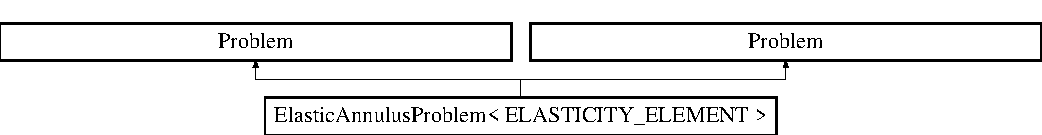
\includegraphics[height=1.818182cm]{classElasticAnnulusProblem}
\end{center}
\end{figure}
\subsection*{Public Member Functions}
\begin{DoxyCompactItemize}
\item 
\hyperlink{classElasticAnnulusProblem_aedf3d30576ccc20e2d8aa809cf075228}{Elastic\+Annulus\+Problem} ()
\begin{DoxyCompactList}\small\item\em Constructor\+: \end{DoxyCompactList}\item 
\hyperlink{classElasticAnnulusProblem_a7e791acd99dc0ae25ab9f2e2fd07c587}{$\sim$\+Elastic\+Annulus\+Problem} ()
\begin{DoxyCompactList}\small\item\em Destructor (empty) \end{DoxyCompactList}\item 
void \hyperlink{classElasticAnnulusProblem_adfb87876ac9981899c6c0b4caf0786f9}{actions\+\_\+after\+\_\+newton\+\_\+solve} ()
\begin{DoxyCompactList}\small\item\em Update function (empty) \end{DoxyCompactList}\item 
void \hyperlink{classElasticAnnulusProblem_af50a0dc2601e1a5e884166941d2cb9ce}{actions\+\_\+before\+\_\+newton\+\_\+solve} ()
\begin{DoxyCompactList}\small\item\em Update function (empty) \end{DoxyCompactList}\item 
void \hyperlink{classElasticAnnulusProblem_a0d2b0cc613caaca7c8f1a78c80b40bc7}{create\+\_\+pml\+\_\+meshes} ()
\begin{DoxyCompactList}\small\item\em Create P\+ML meshes. \end{DoxyCompactList}\item 
void \hyperlink{classElasticAnnulusProblem_abc8f38dd49a37b06212c168588301900}{actions\+\_\+before\+\_\+adapt} ()
\begin{DoxyCompactList}\small\item\em Actions before adapt\+: Wipe the mesh of traction elements. \end{DoxyCompactList}\item 
void \hyperlink{classElasticAnnulusProblem_aa47beeedeac662b19c0f992daf77ef25}{actions\+\_\+after\+\_\+adapt} ()
\begin{DoxyCompactList}\small\item\em Actions after adapt\+: Rebuild the mesh of traction elements. \end{DoxyCompactList}\item 
void \hyperlink{classElasticAnnulusProblem_ab2952a8591047f62f9f66cfe29a533de}{doc\+\_\+solution} (Doc\+Info \&doc\+\_\+info)
\begin{DoxyCompactList}\small\item\em Doc the solution. \end{DoxyCompactList}\item 
\hyperlink{classElasticAnnulusProblem_aedf3d30576ccc20e2d8aa809cf075228}{Elastic\+Annulus\+Problem} ()
\begin{DoxyCompactList}\small\item\em Constructor\+: \end{DoxyCompactList}\item 
\hyperlink{classElasticAnnulusProblem_a7e791acd99dc0ae25ab9f2e2fd07c587}{$\sim$\+Elastic\+Annulus\+Problem} ()
\begin{DoxyCompactList}\small\item\em Destructor (empty) \end{DoxyCompactList}\item 
void \hyperlink{classElasticAnnulusProblem_adfb87876ac9981899c6c0b4caf0786f9}{actions\+\_\+after\+\_\+newton\+\_\+solve} ()
\begin{DoxyCompactList}\small\item\em Update function (empty) \end{DoxyCompactList}\item 
void \hyperlink{classElasticAnnulusProblem_af50a0dc2601e1a5e884166941d2cb9ce}{actions\+\_\+before\+\_\+newton\+\_\+solve} ()
\begin{DoxyCompactList}\small\item\em Update function (empty) \end{DoxyCompactList}\item 
void \hyperlink{classElasticAnnulusProblem_a0d2b0cc613caaca7c8f1a78c80b40bc7}{create\+\_\+pml\+\_\+meshes} ()
\begin{DoxyCompactList}\small\item\em Create P\+ML meshes. \end{DoxyCompactList}\item 
void \hyperlink{classElasticAnnulusProblem_abc8f38dd49a37b06212c168588301900}{actions\+\_\+before\+\_\+adapt} ()
\begin{DoxyCompactList}\small\item\em Actions before adapt\+: Wipe the mesh of traction elements. \end{DoxyCompactList}\item 
void \hyperlink{classElasticAnnulusProblem_aa47beeedeac662b19c0f992daf77ef25}{actions\+\_\+after\+\_\+adapt} ()
\begin{DoxyCompactList}\small\item\em Actions after adapt\+: Rebuild the mesh of traction elements. \end{DoxyCompactList}\item 
void \hyperlink{classElasticAnnulusProblem_ab2952a8591047f62f9f66cfe29a533de}{doc\+\_\+solution} (Doc\+Info \&doc\+\_\+info)
\begin{DoxyCompactList}\small\item\em Doc the solution. \end{DoxyCompactList}\end{DoxyCompactItemize}
\subsection*{Private Member Functions}
\begin{DoxyCompactItemize}
\item 
void \hyperlink{classElasticAnnulusProblem_a06d509ff3316e5f3072ad5f9144cc33f}{complete\+\_\+problem\+\_\+setup} ()
\begin{DoxyCompactList}\small\item\em Helper function to complete problem setup. \end{DoxyCompactList}\item 
void \hyperlink{classElasticAnnulusProblem_a06d509ff3316e5f3072ad5f9144cc33f}{complete\+\_\+problem\+\_\+setup} ()
\begin{DoxyCompactList}\small\item\em Helper function to complete problem setup. \end{DoxyCompactList}\end{DoxyCompactItemize}
\subsection*{Private Attributes}
\begin{DoxyCompactItemize}
\item 
Refineable\+Triangle\+Mesh$<$ E\+L\+A\+S\+T\+I\+C\+I\+T\+Y\+\_\+\+E\+L\+E\+M\+E\+NT $>$ $\ast$ \hyperlink{classElasticAnnulusProblem_a1e751b41cfaf6314fd93d8b79fbd6d0b}{Solid\+\_\+mesh\+\_\+pt}
\begin{DoxyCompactList}\small\item\em Pointer to refineable solid mesh. \end{DoxyCompactList}\item 
Triangle\+Mesh$<$ E\+L\+A\+S\+T\+I\+C\+I\+T\+Y\+\_\+\+E\+L\+E\+M\+E\+NT $>$ $\ast$ \hyperlink{classElasticAnnulusProblem_af1f36137c361d10c5a474ae186ecad3b}{Solid\+\_\+mesh\+\_\+pt}
\begin{DoxyCompactList}\small\item\em Pointer to solid mesh. \end{DoxyCompactList}\item 
Mesh $\ast$ \hyperlink{classElasticAnnulusProblem_aee24a0070e6010553756a66fd3e609b3}{P\+M\+L\+\_\+right\+\_\+mesh\+\_\+pt}
\begin{DoxyCompactList}\small\item\em Pointer to the right P\+ML mesh. \end{DoxyCompactList}\item 
Mesh $\ast$ \hyperlink{classElasticAnnulusProblem_a2dee4b212d38fb433c412ae6f1fb4c89}{P\+M\+L\+\_\+top\+\_\+mesh\+\_\+pt}
\begin{DoxyCompactList}\small\item\em Pointer to the top P\+ML mesh. \end{DoxyCompactList}\item 
Mesh $\ast$ \hyperlink{classElasticAnnulusProblem_a3498ed82cd25951598b22f3b61136556}{P\+M\+L\+\_\+left\+\_\+mesh\+\_\+pt}
\begin{DoxyCompactList}\small\item\em Pointer to the left P\+ML mesh. \end{DoxyCompactList}\item 
Mesh $\ast$ \hyperlink{classElasticAnnulusProblem_a3307dda934f6cb7bc0615db7eb5b717b}{P\+M\+L\+\_\+bottom\+\_\+mesh\+\_\+pt}
\begin{DoxyCompactList}\small\item\em Pointer to the bottom P\+ML mesh. \end{DoxyCompactList}\item 
Mesh $\ast$ \hyperlink{classElasticAnnulusProblem_a508de7ec878f9b32c279623c1dad31fd}{P\+M\+L\+\_\+top\+\_\+right\+\_\+mesh\+\_\+pt}
\begin{DoxyCompactList}\small\item\em Pointer to the top right corner P\+ML mesh. \end{DoxyCompactList}\item 
Mesh $\ast$ \hyperlink{classElasticAnnulusProblem_ad1c027ba9ff28ce9d9fda09273721ef3}{P\+M\+L\+\_\+top\+\_\+left\+\_\+mesh\+\_\+pt}
\begin{DoxyCompactList}\small\item\em Pointer to the top left corner P\+ML mesh. \end{DoxyCompactList}\item 
Mesh $\ast$ \hyperlink{classElasticAnnulusProblem_a220bc42fa49c06f91810f59eb83f8526}{P\+M\+L\+\_\+bottom\+\_\+right\+\_\+mesh\+\_\+pt}
\begin{DoxyCompactList}\small\item\em Pointer to the bottom right corner P\+ML mesh. \end{DoxyCompactList}\item 
Mesh $\ast$ \hyperlink{classElasticAnnulusProblem_a34551d6f7265da8cc2a1657fa0d605a0}{P\+M\+L\+\_\+bottom\+\_\+left\+\_\+mesh\+\_\+pt}
\begin{DoxyCompactList}\small\item\em Pointer to the bottom left corner P\+ML mesh. \end{DoxyCompactList}\item 
Doc\+Info \hyperlink{classElasticAnnulusProblem_a7d98599c2867fda5aab1719292c4623d}{Doc\+\_\+info}
\begin{DoxyCompactList}\small\item\em Doc\+Info object for output. \end{DoxyCompactList}\item 
unsigned \hyperlink{classElasticAnnulusProblem_af7228afd4d413dfd09e7a4b5bccedd64}{Upper\+\_\+inner\+\_\+boundary\+\_\+id}
\begin{DoxyCompactList}\small\item\em Boundary ID of upper inner boundary. \end{DoxyCompactList}\item 
unsigned \hyperlink{classElasticAnnulusProblem_a30ffabbfca663989fe1e787ff7ec21ba}{Upper\+\_\+outer\+\_\+boundary\+\_\+id}
\begin{DoxyCompactList}\small\item\em Boundary ID of upper outer boundary. \end{DoxyCompactList}\item 
unsigned \hyperlink{classElasticAnnulusProblem_a810f81246ad9ffdc4206016bfb8a56da}{Lower\+\_\+inner\+\_\+boundary\+\_\+id}
\begin{DoxyCompactList}\small\item\em Boundary ID of lower inner boundary. \end{DoxyCompactList}\item 
unsigned \hyperlink{classElasticAnnulusProblem_a21dfc08e2f80d32b674670b1194f7386}{Lower\+\_\+outer\+\_\+boundary\+\_\+id}
\begin{DoxyCompactList}\small\item\em Boundary ID of lower outer boundary. \end{DoxyCompactList}\item 
Rectangular\+Quad\+Mesh$<$ E\+L\+A\+S\+T\+I\+C\+I\+T\+Y\+\_\+\+E\+L\+E\+M\+E\+NT $>$ $\ast$ \hyperlink{classElasticAnnulusProblem_af0c334a5413eac6077177769b2a5f1f8}{Solid\+\_\+mesh\+\_\+pt}
\begin{DoxyCompactList}\small\item\em Pointer to solid mesh. \end{DoxyCompactList}\end{DoxyCompactItemize}


\subsection{Detailed Description}
\subsubsection*{template$<$class E\+L\+A\+S\+T\+I\+C\+I\+T\+Y\+\_\+\+E\+L\+E\+M\+E\+NT$>$\newline
class Elastic\+Annulus\+Problem$<$ E\+L\+A\+S\+T\+I\+C\+I\+T\+Y\+\_\+\+E\+L\+E\+M\+E\+N\+T $>$}

Annular disk. 

Definition at line 248 of file time\+\_\+harmonic\+\_\+elasticity\+\_\+driver.\+cc.



\subsection{Constructor \& Destructor Documentation}
\mbox{\Hypertarget{classElasticAnnulusProblem_aedf3d30576ccc20e2d8aa809cf075228}\label{classElasticAnnulusProblem_aedf3d30576ccc20e2d8aa809cf075228}} 
\index{Elastic\+Annulus\+Problem@{Elastic\+Annulus\+Problem}!Elastic\+Annulus\+Problem@{Elastic\+Annulus\+Problem}}
\index{Elastic\+Annulus\+Problem@{Elastic\+Annulus\+Problem}!Elastic\+Annulus\+Problem@{Elastic\+Annulus\+Problem}}
\subsubsection{\texorpdfstring{Elastic\+Annulus\+Problem()}{ElasticAnnulusProblem()}\hspace{0.1cm}{\footnotesize\ttfamily [1/2]}}
{\footnotesize\ttfamily template$<$class E\+L\+A\+S\+T\+I\+C\+I\+T\+Y\+\_\+\+E\+L\+E\+M\+E\+NT $>$ \\
\hyperlink{classElasticAnnulusProblem}{Elastic\+Annulus\+Problem}$<$ E\+L\+A\+S\+T\+I\+C\+I\+T\+Y\+\_\+\+E\+L\+E\+M\+E\+NT $>$\+::\hyperlink{classElasticAnnulusProblem}{Elastic\+Annulus\+Problem} (\begin{DoxyParamCaption}{ }\end{DoxyParamCaption})}



Constructor\+: 

Number of elements in x direction in the bulk mesh

Number of elements in y direction in the bulk mesh

Start and end spatial coordinates of the bulk mesh in x direction

Start and end spatial coordinates of the bulk mesh in y direction 

Definition at line 340 of file time\+\_\+harmonic\+\_\+elasticity\+\_\+driver.\+cc.



References Global\+\_\+\+Parameters\+::\+Directory, and Global\+\_\+\+Parameters\+::\+Element\+\_\+area.

\mbox{\Hypertarget{classElasticAnnulusProblem_a7e791acd99dc0ae25ab9f2e2fd07c587}\label{classElasticAnnulusProblem_a7e791acd99dc0ae25ab9f2e2fd07c587}} 
\index{Elastic\+Annulus\+Problem@{Elastic\+Annulus\+Problem}!````~Elastic\+Annulus\+Problem@{$\sim$\+Elastic\+Annulus\+Problem}}
\index{````~Elastic\+Annulus\+Problem@{$\sim$\+Elastic\+Annulus\+Problem}!Elastic\+Annulus\+Problem@{Elastic\+Annulus\+Problem}}
\subsubsection{\texorpdfstring{$\sim$\+Elastic\+Annulus\+Problem()}{~ElasticAnnulusProblem()}\hspace{0.1cm}{\footnotesize\ttfamily [1/2]}}
{\footnotesize\ttfamily template$<$class E\+L\+A\+S\+T\+I\+C\+I\+T\+Y\+\_\+\+E\+L\+E\+M\+E\+NT$>$ \\
\hyperlink{classElasticAnnulusProblem}{Elastic\+Annulus\+Problem}$<$ E\+L\+A\+S\+T\+I\+C\+I\+T\+Y\+\_\+\+E\+L\+E\+M\+E\+NT $>$\+::$\sim$\hyperlink{classElasticAnnulusProblem}{Elastic\+Annulus\+Problem} (\begin{DoxyParamCaption}{ }\end{DoxyParamCaption})\hspace{0.3cm}{\ttfamily [inline]}}



Destructor (empty) 



Definition at line 257 of file time\+\_\+harmonic\+\_\+elasticity\+\_\+driver.\+cc.

\mbox{\Hypertarget{classElasticAnnulusProblem_aedf3d30576ccc20e2d8aa809cf075228}\label{classElasticAnnulusProblem_aedf3d30576ccc20e2d8aa809cf075228}} 
\index{Elastic\+Annulus\+Problem@{Elastic\+Annulus\+Problem}!Elastic\+Annulus\+Problem@{Elastic\+Annulus\+Problem}}
\index{Elastic\+Annulus\+Problem@{Elastic\+Annulus\+Problem}!Elastic\+Annulus\+Problem@{Elastic\+Annulus\+Problem}}
\subsubsection{\texorpdfstring{Elastic\+Annulus\+Problem()}{ElasticAnnulusProblem()}\hspace{0.1cm}{\footnotesize\ttfamily [2/2]}}
{\footnotesize\ttfamily template$<$class E\+L\+A\+S\+T\+I\+C\+I\+T\+Y\+\_\+\+E\+L\+E\+M\+E\+NT$>$ \\
\hyperlink{classElasticAnnulusProblem}{Elastic\+Annulus\+Problem}$<$ E\+L\+A\+S\+T\+I\+C\+I\+T\+Y\+\_\+\+E\+L\+E\+M\+E\+NT $>$\+::\hyperlink{classElasticAnnulusProblem}{Elastic\+Annulus\+Problem} (\begin{DoxyParamCaption}{ }\end{DoxyParamCaption})}



Constructor\+: 

\mbox{\Hypertarget{classElasticAnnulusProblem_a7e791acd99dc0ae25ab9f2e2fd07c587}\label{classElasticAnnulusProblem_a7e791acd99dc0ae25ab9f2e2fd07c587}} 
\index{Elastic\+Annulus\+Problem@{Elastic\+Annulus\+Problem}!````~Elastic\+Annulus\+Problem@{$\sim$\+Elastic\+Annulus\+Problem}}
\index{````~Elastic\+Annulus\+Problem@{$\sim$\+Elastic\+Annulus\+Problem}!Elastic\+Annulus\+Problem@{Elastic\+Annulus\+Problem}}
\subsubsection{\texorpdfstring{$\sim$\+Elastic\+Annulus\+Problem()}{~ElasticAnnulusProblem()}\hspace{0.1cm}{\footnotesize\ttfamily [2/2]}}
{\footnotesize\ttfamily template$<$class E\+L\+A\+S\+T\+I\+C\+I\+T\+Y\+\_\+\+E\+L\+E\+M\+E\+NT$>$ \\
\hyperlink{classElasticAnnulusProblem}{Elastic\+Annulus\+Problem}$<$ E\+L\+A\+S\+T\+I\+C\+I\+T\+Y\+\_\+\+E\+L\+E\+M\+E\+NT $>$\+::$\sim$\hyperlink{classElasticAnnulusProblem}{Elastic\+Annulus\+Problem} (\begin{DoxyParamCaption}{ }\end{DoxyParamCaption})\hspace{0.3cm}{\ttfamily [inline]}}



Destructor (empty) 



Definition at line 154 of file time\+\_\+harmonic\+\_\+elasticity\+\_\+driver\+\_\+source.\+cc.



\subsection{Member Function Documentation}
\mbox{\Hypertarget{classElasticAnnulusProblem_aa47beeedeac662b19c0f992daf77ef25}\label{classElasticAnnulusProblem_aa47beeedeac662b19c0f992daf77ef25}} 
\index{Elastic\+Annulus\+Problem@{Elastic\+Annulus\+Problem}!actions\+\_\+after\+\_\+adapt@{actions\+\_\+after\+\_\+adapt}}
\index{actions\+\_\+after\+\_\+adapt@{actions\+\_\+after\+\_\+adapt}!Elastic\+Annulus\+Problem@{Elastic\+Annulus\+Problem}}
\subsubsection{\texorpdfstring{actions\+\_\+after\+\_\+adapt()}{actions\_after\_adapt()}\hspace{0.1cm}{\footnotesize\ttfamily [1/2]}}
{\footnotesize\ttfamily template$<$class E\+L\+A\+S\+T\+I\+C\+I\+T\+Y\+\_\+\+E\+L\+E\+M\+E\+NT$>$ \\
void \hyperlink{classElasticAnnulusProblem}{Elastic\+Annulus\+Problem}$<$ E\+L\+A\+S\+T\+I\+C\+I\+T\+Y\+\_\+\+E\+L\+E\+M\+E\+NT $>$\+::actions\+\_\+after\+\_\+adapt (\begin{DoxyParamCaption}{ }\end{DoxyParamCaption})}



Actions after adapt\+: Rebuild the mesh of traction elements. 

\mbox{\Hypertarget{classElasticAnnulusProblem_aa47beeedeac662b19c0f992daf77ef25}\label{classElasticAnnulusProblem_aa47beeedeac662b19c0f992daf77ef25}} 
\index{Elastic\+Annulus\+Problem@{Elastic\+Annulus\+Problem}!actions\+\_\+after\+\_\+adapt@{actions\+\_\+after\+\_\+adapt}}
\index{actions\+\_\+after\+\_\+adapt@{actions\+\_\+after\+\_\+adapt}!Elastic\+Annulus\+Problem@{Elastic\+Annulus\+Problem}}
\subsubsection{\texorpdfstring{actions\+\_\+after\+\_\+adapt()}{actions\_after\_adapt()}\hspace{0.1cm}{\footnotesize\ttfamily [2/2]}}
{\footnotesize\ttfamily template$<$class E\+L\+A\+S\+T\+I\+C\+I\+T\+Y\+\_\+\+E\+L\+E\+M\+E\+NT $>$ \\
void \hyperlink{classElasticAnnulusProblem}{Elastic\+Annulus\+Problem}$<$ E\+L\+A\+S\+T\+I\+C\+I\+T\+Y\+\_\+\+E\+L\+E\+M\+E\+NT $>$\+::actions\+\_\+after\+\_\+adapt (\begin{DoxyParamCaption}{ }\end{DoxyParamCaption})}



Actions after adapt\+: Rebuild the mesh of traction elements. 

Actions after adapt\+: complete problem setup. 

Definition at line 615 of file time\+\_\+harmonic\+\_\+elasticity\+\_\+driver.\+cc.

\mbox{\Hypertarget{classElasticAnnulusProblem_adfb87876ac9981899c6c0b4caf0786f9}\label{classElasticAnnulusProblem_adfb87876ac9981899c6c0b4caf0786f9}} 
\index{Elastic\+Annulus\+Problem@{Elastic\+Annulus\+Problem}!actions\+\_\+after\+\_\+newton\+\_\+solve@{actions\+\_\+after\+\_\+newton\+\_\+solve}}
\index{actions\+\_\+after\+\_\+newton\+\_\+solve@{actions\+\_\+after\+\_\+newton\+\_\+solve}!Elastic\+Annulus\+Problem@{Elastic\+Annulus\+Problem}}
\subsubsection{\texorpdfstring{actions\+\_\+after\+\_\+newton\+\_\+solve()}{actions\_after\_newton\_solve()}\hspace{0.1cm}{\footnotesize\ttfamily [1/2]}}
{\footnotesize\ttfamily template$<$class E\+L\+A\+S\+T\+I\+C\+I\+T\+Y\+\_\+\+E\+L\+E\+M\+E\+NT$>$ \\
void \hyperlink{classElasticAnnulusProblem}{Elastic\+Annulus\+Problem}$<$ E\+L\+A\+S\+T\+I\+C\+I\+T\+Y\+\_\+\+E\+L\+E\+M\+E\+NT $>$\+::actions\+\_\+after\+\_\+newton\+\_\+solve (\begin{DoxyParamCaption}{ }\end{DoxyParamCaption})\hspace{0.3cm}{\ttfamily [inline]}}



Update function (empty) 



Definition at line 157 of file time\+\_\+harmonic\+\_\+elasticity\+\_\+driver\+\_\+source.\+cc.

\mbox{\Hypertarget{classElasticAnnulusProblem_adfb87876ac9981899c6c0b4caf0786f9}\label{classElasticAnnulusProblem_adfb87876ac9981899c6c0b4caf0786f9}} 
\index{Elastic\+Annulus\+Problem@{Elastic\+Annulus\+Problem}!actions\+\_\+after\+\_\+newton\+\_\+solve@{actions\+\_\+after\+\_\+newton\+\_\+solve}}
\index{actions\+\_\+after\+\_\+newton\+\_\+solve@{actions\+\_\+after\+\_\+newton\+\_\+solve}!Elastic\+Annulus\+Problem@{Elastic\+Annulus\+Problem}}
\subsubsection{\texorpdfstring{actions\+\_\+after\+\_\+newton\+\_\+solve()}{actions\_after\_newton\_solve()}\hspace{0.1cm}{\footnotesize\ttfamily [2/2]}}
{\footnotesize\ttfamily template$<$class E\+L\+A\+S\+T\+I\+C\+I\+T\+Y\+\_\+\+E\+L\+E\+M\+E\+NT$>$ \\
void \hyperlink{classElasticAnnulusProblem}{Elastic\+Annulus\+Problem}$<$ E\+L\+A\+S\+T\+I\+C\+I\+T\+Y\+\_\+\+E\+L\+E\+M\+E\+NT $>$\+::actions\+\_\+after\+\_\+newton\+\_\+solve (\begin{DoxyParamCaption}{ }\end{DoxyParamCaption})\hspace{0.3cm}{\ttfamily [inline]}}



Update function (empty) 



Definition at line 260 of file time\+\_\+harmonic\+\_\+elasticity\+\_\+driver.\+cc.

\mbox{\Hypertarget{classElasticAnnulusProblem_abc8f38dd49a37b06212c168588301900}\label{classElasticAnnulusProblem_abc8f38dd49a37b06212c168588301900}} 
\index{Elastic\+Annulus\+Problem@{Elastic\+Annulus\+Problem}!actions\+\_\+before\+\_\+adapt@{actions\+\_\+before\+\_\+adapt}}
\index{actions\+\_\+before\+\_\+adapt@{actions\+\_\+before\+\_\+adapt}!Elastic\+Annulus\+Problem@{Elastic\+Annulus\+Problem}}
\subsubsection{\texorpdfstring{actions\+\_\+before\+\_\+adapt()}{actions\_before\_adapt()}\hspace{0.1cm}{\footnotesize\ttfamily [1/2]}}
{\footnotesize\ttfamily template$<$class E\+L\+A\+S\+T\+I\+C\+I\+T\+Y\+\_\+\+E\+L\+E\+M\+E\+NT$>$ \\
void \hyperlink{classElasticAnnulusProblem}{Elastic\+Annulus\+Problem}$<$ E\+L\+A\+S\+T\+I\+C\+I\+T\+Y\+\_\+\+E\+L\+E\+M\+E\+NT $>$\+::actions\+\_\+before\+\_\+adapt (\begin{DoxyParamCaption}{ }\end{DoxyParamCaption})}



Actions before adapt\+: Wipe the mesh of traction elements. 

\mbox{\Hypertarget{classElasticAnnulusProblem_abc8f38dd49a37b06212c168588301900}\label{classElasticAnnulusProblem_abc8f38dd49a37b06212c168588301900}} 
\index{Elastic\+Annulus\+Problem@{Elastic\+Annulus\+Problem}!actions\+\_\+before\+\_\+adapt@{actions\+\_\+before\+\_\+adapt}}
\index{actions\+\_\+before\+\_\+adapt@{actions\+\_\+before\+\_\+adapt}!Elastic\+Annulus\+Problem@{Elastic\+Annulus\+Problem}}
\subsubsection{\texorpdfstring{actions\+\_\+before\+\_\+adapt()}{actions\_before\_adapt()}\hspace{0.1cm}{\footnotesize\ttfamily [2/2]}}
{\footnotesize\ttfamily template$<$class E\+L\+A\+S\+T\+I\+C\+I\+T\+Y\+\_\+\+E\+L\+E\+M\+E\+NT $>$ \\
void \hyperlink{classElasticAnnulusProblem}{Elastic\+Annulus\+Problem}$<$ E\+L\+A\+S\+T\+I\+C\+I\+T\+Y\+\_\+\+E\+L\+E\+M\+E\+NT $>$\+::actions\+\_\+before\+\_\+adapt (\begin{DoxyParamCaption}{ }\end{DoxyParamCaption})}



Actions before adapt\+: Wipe the mesh of traction elements. 

Actions before adapt\+: empty. 

Definition at line 575 of file time\+\_\+harmonic\+\_\+elasticity\+\_\+driver.\+cc.

\mbox{\Hypertarget{classElasticAnnulusProblem_af50a0dc2601e1a5e884166941d2cb9ce}\label{classElasticAnnulusProblem_af50a0dc2601e1a5e884166941d2cb9ce}} 
\index{Elastic\+Annulus\+Problem@{Elastic\+Annulus\+Problem}!actions\+\_\+before\+\_\+newton\+\_\+solve@{actions\+\_\+before\+\_\+newton\+\_\+solve}}
\index{actions\+\_\+before\+\_\+newton\+\_\+solve@{actions\+\_\+before\+\_\+newton\+\_\+solve}!Elastic\+Annulus\+Problem@{Elastic\+Annulus\+Problem}}
\subsubsection{\texorpdfstring{actions\+\_\+before\+\_\+newton\+\_\+solve()}{actions\_before\_newton\_solve()}\hspace{0.1cm}{\footnotesize\ttfamily [1/2]}}
{\footnotesize\ttfamily template$<$class E\+L\+A\+S\+T\+I\+C\+I\+T\+Y\+\_\+\+E\+L\+E\+M\+E\+NT$>$ \\
void \hyperlink{classElasticAnnulusProblem}{Elastic\+Annulus\+Problem}$<$ E\+L\+A\+S\+T\+I\+C\+I\+T\+Y\+\_\+\+E\+L\+E\+M\+E\+NT $>$\+::actions\+\_\+before\+\_\+newton\+\_\+solve (\begin{DoxyParamCaption}{ }\end{DoxyParamCaption})\hspace{0.3cm}{\ttfamily [inline]}}



Update function (empty) 



Definition at line 160 of file time\+\_\+harmonic\+\_\+elasticity\+\_\+driver\+\_\+source.\+cc.

\mbox{\Hypertarget{classElasticAnnulusProblem_af50a0dc2601e1a5e884166941d2cb9ce}\label{classElasticAnnulusProblem_af50a0dc2601e1a5e884166941d2cb9ce}} 
\index{Elastic\+Annulus\+Problem@{Elastic\+Annulus\+Problem}!actions\+\_\+before\+\_\+newton\+\_\+solve@{actions\+\_\+before\+\_\+newton\+\_\+solve}}
\index{actions\+\_\+before\+\_\+newton\+\_\+solve@{actions\+\_\+before\+\_\+newton\+\_\+solve}!Elastic\+Annulus\+Problem@{Elastic\+Annulus\+Problem}}
\subsubsection{\texorpdfstring{actions\+\_\+before\+\_\+newton\+\_\+solve()}{actions\_before\_newton\_solve()}\hspace{0.1cm}{\footnotesize\ttfamily [2/2]}}
{\footnotesize\ttfamily template$<$class E\+L\+A\+S\+T\+I\+C\+I\+T\+Y\+\_\+\+E\+L\+E\+M\+E\+NT$>$ \\
void \hyperlink{classElasticAnnulusProblem}{Elastic\+Annulus\+Problem}$<$ E\+L\+A\+S\+T\+I\+C\+I\+T\+Y\+\_\+\+E\+L\+E\+M\+E\+NT $>$\+::actions\+\_\+before\+\_\+newton\+\_\+solve (\begin{DoxyParamCaption}{ }\end{DoxyParamCaption})\hspace{0.3cm}{\ttfamily [inline]}}



Update function (empty) 



Definition at line 263 of file time\+\_\+harmonic\+\_\+elasticity\+\_\+driver.\+cc.

\mbox{\Hypertarget{classElasticAnnulusProblem_a06d509ff3316e5f3072ad5f9144cc33f}\label{classElasticAnnulusProblem_a06d509ff3316e5f3072ad5f9144cc33f}} 
\index{Elastic\+Annulus\+Problem@{Elastic\+Annulus\+Problem}!complete\+\_\+problem\+\_\+setup@{complete\+\_\+problem\+\_\+setup}}
\index{complete\+\_\+problem\+\_\+setup@{complete\+\_\+problem\+\_\+setup}!Elastic\+Annulus\+Problem@{Elastic\+Annulus\+Problem}}
\subsubsection{\texorpdfstring{complete\+\_\+problem\+\_\+setup()}{complete\_problem\_setup()}\hspace{0.1cm}{\footnotesize\ttfamily [1/2]}}
{\footnotesize\ttfamily template$<$class E\+L\+A\+S\+T\+I\+C\+I\+T\+Y\+\_\+\+E\+L\+E\+M\+E\+NT$>$ \\
void \hyperlink{classElasticAnnulusProblem}{Elastic\+Annulus\+Problem}$<$ E\+L\+A\+S\+T\+I\+C\+I\+T\+Y\+\_\+\+E\+L\+E\+M\+E\+NT $>$\+::complete\+\_\+problem\+\_\+setup (\begin{DoxyParamCaption}{ }\end{DoxyParamCaption})\hspace{0.3cm}{\ttfamily [private]}}



Helper function to complete problem setup. 

\mbox{\Hypertarget{classElasticAnnulusProblem_a06d509ff3316e5f3072ad5f9144cc33f}\label{classElasticAnnulusProblem_a06d509ff3316e5f3072ad5f9144cc33f}} 
\index{Elastic\+Annulus\+Problem@{Elastic\+Annulus\+Problem}!complete\+\_\+problem\+\_\+setup@{complete\+\_\+problem\+\_\+setup}}
\index{complete\+\_\+problem\+\_\+setup@{complete\+\_\+problem\+\_\+setup}!Elastic\+Annulus\+Problem@{Elastic\+Annulus\+Problem}}
\subsubsection{\texorpdfstring{complete\+\_\+problem\+\_\+setup()}{complete\_problem\_setup()}\hspace{0.1cm}{\footnotesize\ttfamily [2/2]}}
{\footnotesize\ttfamily template$<$class E\+L\+A\+S\+T\+I\+C\+I\+T\+Y\+\_\+\+E\+L\+E\+M\+E\+NT $>$ \\
void \hyperlink{classElasticAnnulusProblem}{Elastic\+Annulus\+Problem}$<$ E\+L\+A\+S\+T\+I\+C\+I\+T\+Y\+\_\+\+E\+L\+E\+M\+E\+NT $>$\+::complete\+\_\+problem\+\_\+setup (\begin{DoxyParamCaption}{ }\end{DoxyParamCaption})\hspace{0.3cm}{\ttfamily [private]}}



Helper function to complete problem setup. 

Complete problem setup. Upcast from P\+M\+L\+Element to time harmonic linear elasticity bulk element

Boundaries with id 0 and 1 represent the interior boundary and these are the only ones that need to be processed, hence the loop below only considers nodes on these two boundaries. 

Definition at line 516 of file time\+\_\+harmonic\+\_\+elasticity\+\_\+driver.\+cc.



References Global\+\_\+\+Parameters\+::\+E\+\_\+pt, Global\+\_\+\+Parameters\+::exact\+\_\+u(), and Global\+\_\+\+Parameters\+::\+Omega\+\_\+sq.

\mbox{\Hypertarget{classElasticAnnulusProblem_a0d2b0cc613caaca7c8f1a78c80b40bc7}\label{classElasticAnnulusProblem_a0d2b0cc613caaca7c8f1a78c80b40bc7}} 
\index{Elastic\+Annulus\+Problem@{Elastic\+Annulus\+Problem}!create\+\_\+pml\+\_\+meshes@{create\+\_\+pml\+\_\+meshes}}
\index{create\+\_\+pml\+\_\+meshes@{create\+\_\+pml\+\_\+meshes}!Elastic\+Annulus\+Problem@{Elastic\+Annulus\+Problem}}
\subsubsection{\texorpdfstring{create\+\_\+pml\+\_\+meshes()}{create\_pml\_meshes()}\hspace{0.1cm}{\footnotesize\ttfamily [1/2]}}
{\footnotesize\ttfamily template$<$class E\+L\+A\+S\+T\+I\+C\+I\+T\+Y\+\_\+\+E\+L\+E\+M\+E\+NT$>$ \\
void \hyperlink{classElasticAnnulusProblem}{Elastic\+Annulus\+Problem}$<$ E\+L\+A\+S\+T\+I\+C\+I\+T\+Y\+\_\+\+E\+L\+E\+M\+E\+NT $>$\+::create\+\_\+pml\+\_\+meshes (\begin{DoxyParamCaption}{ }\end{DoxyParamCaption})}



Create P\+ML meshes. 

\mbox{\Hypertarget{classElasticAnnulusProblem_a0d2b0cc613caaca7c8f1a78c80b40bc7}\label{classElasticAnnulusProblem_a0d2b0cc613caaca7c8f1a78c80b40bc7}} 
\index{Elastic\+Annulus\+Problem@{Elastic\+Annulus\+Problem}!create\+\_\+pml\+\_\+meshes@{create\+\_\+pml\+\_\+meshes}}
\index{create\+\_\+pml\+\_\+meshes@{create\+\_\+pml\+\_\+meshes}!Elastic\+Annulus\+Problem@{Elastic\+Annulus\+Problem}}
\subsubsection{\texorpdfstring{create\+\_\+pml\+\_\+meshes()}{create\_pml\_meshes()}\hspace{0.1cm}{\footnotesize\ttfamily [2/2]}}
{\footnotesize\ttfamily template$<$class E\+L\+A\+S\+T\+I\+C\+I\+T\+Y\+\_\+\+E\+L\+E\+M\+E\+NT $>$ \\
void \hyperlink{classElasticAnnulusProblem}{Elastic\+Annulus\+Problem}$<$ E\+L\+A\+S\+T\+I\+C\+I\+T\+Y\+\_\+\+E\+L\+E\+M\+E\+NT $>$\+::create\+\_\+pml\+\_\+meshes (\begin{DoxyParamCaption}{ }\end{DoxyParamCaption})}



Create P\+ML meshes. 

Create P\+ML meshes and add them to the problem\textquotesingle{}s sub-\/meshes. 

Definition at line 756 of file time\+\_\+harmonic\+\_\+elasticity\+\_\+driver.\+cc.



References Global\+\_\+\+Parameters\+::\+N\+\_\+x\+\_\+left\+\_\+pml, Global\+\_\+\+Parameters\+::\+N\+\_\+x\+\_\+right\+\_\+pml, Global\+\_\+\+Parameters\+::\+N\+\_\+y\+\_\+bottom\+\_\+pml, Global\+\_\+\+Parameters\+::\+N\+\_\+y\+\_\+top\+\_\+pml, Global\+\_\+\+Parameters\+::\+Width\+\_\+x\+\_\+left\+\_\+pml, Global\+\_\+\+Parameters\+::\+Width\+\_\+x\+\_\+right\+\_\+pml, Global\+\_\+\+Parameters\+::\+Width\+\_\+y\+\_\+bottom\+\_\+pml, and Global\+\_\+\+Parameters\+::\+Width\+\_\+y\+\_\+top\+\_\+pml.

\mbox{\Hypertarget{classElasticAnnulusProblem_ab2952a8591047f62f9f66cfe29a533de}\label{classElasticAnnulusProblem_ab2952a8591047f62f9f66cfe29a533de}} 
\index{Elastic\+Annulus\+Problem@{Elastic\+Annulus\+Problem}!doc\+\_\+solution@{doc\+\_\+solution}}
\index{doc\+\_\+solution@{doc\+\_\+solution}!Elastic\+Annulus\+Problem@{Elastic\+Annulus\+Problem}}
\subsubsection{\texorpdfstring{doc\+\_\+solution()}{doc\_solution()}\hspace{0.1cm}{\footnotesize\ttfamily [1/2]}}
{\footnotesize\ttfamily template$<$class E\+L\+A\+S\+T\+I\+C\+I\+T\+Y\+\_\+\+E\+L\+E\+M\+E\+NT$>$ \\
void \hyperlink{classElasticAnnulusProblem}{Elastic\+Annulus\+Problem}$<$ E\+L\+A\+S\+T\+I\+C\+I\+T\+Y\+\_\+\+E\+L\+E\+M\+E\+NT $>$\+::doc\+\_\+solution (\begin{DoxyParamCaption}\item[{Doc\+Info \&}]{doc\+\_\+info }\end{DoxyParamCaption})}



Doc the solution. 

\mbox{\Hypertarget{classElasticAnnulusProblem_ab2952a8591047f62f9f66cfe29a533de}\label{classElasticAnnulusProblem_ab2952a8591047f62f9f66cfe29a533de}} 
\index{Elastic\+Annulus\+Problem@{Elastic\+Annulus\+Problem}!doc\+\_\+solution@{doc\+\_\+solution}}
\index{doc\+\_\+solution@{doc\+\_\+solution}!Elastic\+Annulus\+Problem@{Elastic\+Annulus\+Problem}}
\subsubsection{\texorpdfstring{doc\+\_\+solution()}{doc\_solution()}\hspace{0.1cm}{\footnotesize\ttfamily [2/2]}}
{\footnotesize\ttfamily template$<$class E\+L\+A\+S\+T\+I\+C\+I\+T\+Y\+\_\+\+E\+L\+E\+M\+E\+NT $>$ \\
void \hyperlink{classElasticAnnulusProblem}{Elastic\+Annulus\+Problem}$<$ E\+L\+A\+S\+T\+I\+C\+I\+T\+Y\+\_\+\+E\+L\+E\+M\+E\+NT $>$\+::doc\+\_\+solution (\begin{DoxyParamCaption}\item[{Doc\+Info \&}]{doc\+\_\+info }\end{DoxyParamCaption})}



Doc the solution. 



Definition at line 633 of file time\+\_\+harmonic\+\_\+elasticity\+\_\+driver.\+cc.



References Global\+\_\+\+Parameters\+::exact\+\_\+u(), Global\+\_\+\+Parameters\+::\+T\+\_\+end, and Global\+\_\+\+Parameters\+::\+T\+\_\+start.



Referenced by main().



\subsection{Member Data Documentation}
\mbox{\Hypertarget{classElasticAnnulusProblem_a7d98599c2867fda5aab1719292c4623d}\label{classElasticAnnulusProblem_a7d98599c2867fda5aab1719292c4623d}} 
\index{Elastic\+Annulus\+Problem@{Elastic\+Annulus\+Problem}!Doc\+\_\+info@{Doc\+\_\+info}}
\index{Doc\+\_\+info@{Doc\+\_\+info}!Elastic\+Annulus\+Problem@{Elastic\+Annulus\+Problem}}
\subsubsection{\texorpdfstring{Doc\+\_\+info}{Doc\_info}}
{\footnotesize\ttfamily template$<$class E\+L\+A\+S\+T\+I\+C\+I\+T\+Y\+\_\+\+E\+L\+E\+M\+E\+NT$>$ \\
Doc\+Info \hyperlink{classElasticAnnulusProblem}{Elastic\+Annulus\+Problem}$<$ E\+L\+A\+S\+T\+I\+C\+I\+T\+Y\+\_\+\+E\+L\+E\+M\+E\+NT $>$\+::Doc\+\_\+info\hspace{0.3cm}{\ttfamily [private]}}



Doc\+Info object for output. 



Definition at line 319 of file time\+\_\+harmonic\+\_\+elasticity\+\_\+driver.\+cc.

\mbox{\Hypertarget{classElasticAnnulusProblem_a810f81246ad9ffdc4206016bfb8a56da}\label{classElasticAnnulusProblem_a810f81246ad9ffdc4206016bfb8a56da}} 
\index{Elastic\+Annulus\+Problem@{Elastic\+Annulus\+Problem}!Lower\+\_\+inner\+\_\+boundary\+\_\+id@{Lower\+\_\+inner\+\_\+boundary\+\_\+id}}
\index{Lower\+\_\+inner\+\_\+boundary\+\_\+id@{Lower\+\_\+inner\+\_\+boundary\+\_\+id}!Elastic\+Annulus\+Problem@{Elastic\+Annulus\+Problem}}
\subsubsection{\texorpdfstring{Lower\+\_\+inner\+\_\+boundary\+\_\+id}{Lower\_inner\_boundary\_id}}
{\footnotesize\ttfamily template$<$class E\+L\+A\+S\+T\+I\+C\+I\+T\+Y\+\_\+\+E\+L\+E\+M\+E\+NT$>$ \\
unsigned \hyperlink{classElasticAnnulusProblem}{Elastic\+Annulus\+Problem}$<$ E\+L\+A\+S\+T\+I\+C\+I\+T\+Y\+\_\+\+E\+L\+E\+M\+E\+NT $>$\+::Lower\+\_\+inner\+\_\+boundary\+\_\+id\hspace{0.3cm}{\ttfamily [private]}}



Boundary ID of lower inner boundary. 



Definition at line 328 of file time\+\_\+harmonic\+\_\+elasticity\+\_\+driver.\+cc.

\mbox{\Hypertarget{classElasticAnnulusProblem_a21dfc08e2f80d32b674670b1194f7386}\label{classElasticAnnulusProblem_a21dfc08e2f80d32b674670b1194f7386}} 
\index{Elastic\+Annulus\+Problem@{Elastic\+Annulus\+Problem}!Lower\+\_\+outer\+\_\+boundary\+\_\+id@{Lower\+\_\+outer\+\_\+boundary\+\_\+id}}
\index{Lower\+\_\+outer\+\_\+boundary\+\_\+id@{Lower\+\_\+outer\+\_\+boundary\+\_\+id}!Elastic\+Annulus\+Problem@{Elastic\+Annulus\+Problem}}
\subsubsection{\texorpdfstring{Lower\+\_\+outer\+\_\+boundary\+\_\+id}{Lower\_outer\_boundary\_id}}
{\footnotesize\ttfamily template$<$class E\+L\+A\+S\+T\+I\+C\+I\+T\+Y\+\_\+\+E\+L\+E\+M\+E\+NT$>$ \\
unsigned \hyperlink{classElasticAnnulusProblem}{Elastic\+Annulus\+Problem}$<$ E\+L\+A\+S\+T\+I\+C\+I\+T\+Y\+\_\+\+E\+L\+E\+M\+E\+NT $>$\+::Lower\+\_\+outer\+\_\+boundary\+\_\+id\hspace{0.3cm}{\ttfamily [private]}}



Boundary ID of lower outer boundary. 



Definition at line 331 of file time\+\_\+harmonic\+\_\+elasticity\+\_\+driver.\+cc.

\mbox{\Hypertarget{classElasticAnnulusProblem_a34551d6f7265da8cc2a1657fa0d605a0}\label{classElasticAnnulusProblem_a34551d6f7265da8cc2a1657fa0d605a0}} 
\index{Elastic\+Annulus\+Problem@{Elastic\+Annulus\+Problem}!P\+M\+L\+\_\+bottom\+\_\+left\+\_\+mesh\+\_\+pt@{P\+M\+L\+\_\+bottom\+\_\+left\+\_\+mesh\+\_\+pt}}
\index{P\+M\+L\+\_\+bottom\+\_\+left\+\_\+mesh\+\_\+pt@{P\+M\+L\+\_\+bottom\+\_\+left\+\_\+mesh\+\_\+pt}!Elastic\+Annulus\+Problem@{Elastic\+Annulus\+Problem}}
\subsubsection{\texorpdfstring{P\+M\+L\+\_\+bottom\+\_\+left\+\_\+mesh\+\_\+pt}{PML\_bottom\_left\_mesh\_pt}}
{\footnotesize\ttfamily template$<$class E\+L\+A\+S\+T\+I\+C\+I\+T\+Y\+\_\+\+E\+L\+E\+M\+E\+NT$>$ \\
Mesh $\ast$ \hyperlink{classElasticAnnulusProblem}{Elastic\+Annulus\+Problem}$<$ E\+L\+A\+S\+T\+I\+C\+I\+T\+Y\+\_\+\+E\+L\+E\+M\+E\+NT $>$\+::P\+M\+L\+\_\+bottom\+\_\+left\+\_\+mesh\+\_\+pt\hspace{0.3cm}{\ttfamily [private]}}



Pointer to the bottom left corner P\+ML mesh. 



Definition at line 316 of file time\+\_\+harmonic\+\_\+elasticity\+\_\+driver.\+cc.

\mbox{\Hypertarget{classElasticAnnulusProblem_a3307dda934f6cb7bc0615db7eb5b717b}\label{classElasticAnnulusProblem_a3307dda934f6cb7bc0615db7eb5b717b}} 
\index{Elastic\+Annulus\+Problem@{Elastic\+Annulus\+Problem}!P\+M\+L\+\_\+bottom\+\_\+mesh\+\_\+pt@{P\+M\+L\+\_\+bottom\+\_\+mesh\+\_\+pt}}
\index{P\+M\+L\+\_\+bottom\+\_\+mesh\+\_\+pt@{P\+M\+L\+\_\+bottom\+\_\+mesh\+\_\+pt}!Elastic\+Annulus\+Problem@{Elastic\+Annulus\+Problem}}
\subsubsection{\texorpdfstring{P\+M\+L\+\_\+bottom\+\_\+mesh\+\_\+pt}{PML\_bottom\_mesh\_pt}}
{\footnotesize\ttfamily template$<$class E\+L\+A\+S\+T\+I\+C\+I\+T\+Y\+\_\+\+E\+L\+E\+M\+E\+NT$>$ \\
Mesh $\ast$ \hyperlink{classElasticAnnulusProblem}{Elastic\+Annulus\+Problem}$<$ E\+L\+A\+S\+T\+I\+C\+I\+T\+Y\+\_\+\+E\+L\+E\+M\+E\+NT $>$\+::P\+M\+L\+\_\+bottom\+\_\+mesh\+\_\+pt\hspace{0.3cm}{\ttfamily [private]}}



Pointer to the bottom P\+ML mesh. 



Definition at line 304 of file time\+\_\+harmonic\+\_\+elasticity\+\_\+driver.\+cc.

\mbox{\Hypertarget{classElasticAnnulusProblem_a220bc42fa49c06f91810f59eb83f8526}\label{classElasticAnnulusProblem_a220bc42fa49c06f91810f59eb83f8526}} 
\index{Elastic\+Annulus\+Problem@{Elastic\+Annulus\+Problem}!P\+M\+L\+\_\+bottom\+\_\+right\+\_\+mesh\+\_\+pt@{P\+M\+L\+\_\+bottom\+\_\+right\+\_\+mesh\+\_\+pt}}
\index{P\+M\+L\+\_\+bottom\+\_\+right\+\_\+mesh\+\_\+pt@{P\+M\+L\+\_\+bottom\+\_\+right\+\_\+mesh\+\_\+pt}!Elastic\+Annulus\+Problem@{Elastic\+Annulus\+Problem}}
\subsubsection{\texorpdfstring{P\+M\+L\+\_\+bottom\+\_\+right\+\_\+mesh\+\_\+pt}{PML\_bottom\_right\_mesh\_pt}}
{\footnotesize\ttfamily template$<$class E\+L\+A\+S\+T\+I\+C\+I\+T\+Y\+\_\+\+E\+L\+E\+M\+E\+NT$>$ \\
Mesh $\ast$ \hyperlink{classElasticAnnulusProblem}{Elastic\+Annulus\+Problem}$<$ E\+L\+A\+S\+T\+I\+C\+I\+T\+Y\+\_\+\+E\+L\+E\+M\+E\+NT $>$\+::P\+M\+L\+\_\+bottom\+\_\+right\+\_\+mesh\+\_\+pt\hspace{0.3cm}{\ttfamily [private]}}



Pointer to the bottom right corner P\+ML mesh. 



Definition at line 313 of file time\+\_\+harmonic\+\_\+elasticity\+\_\+driver.\+cc.

\mbox{\Hypertarget{classElasticAnnulusProblem_a3498ed82cd25951598b22f3b61136556}\label{classElasticAnnulusProblem_a3498ed82cd25951598b22f3b61136556}} 
\index{Elastic\+Annulus\+Problem@{Elastic\+Annulus\+Problem}!P\+M\+L\+\_\+left\+\_\+mesh\+\_\+pt@{P\+M\+L\+\_\+left\+\_\+mesh\+\_\+pt}}
\index{P\+M\+L\+\_\+left\+\_\+mesh\+\_\+pt@{P\+M\+L\+\_\+left\+\_\+mesh\+\_\+pt}!Elastic\+Annulus\+Problem@{Elastic\+Annulus\+Problem}}
\subsubsection{\texorpdfstring{P\+M\+L\+\_\+left\+\_\+mesh\+\_\+pt}{PML\_left\_mesh\_pt}}
{\footnotesize\ttfamily template$<$class E\+L\+A\+S\+T\+I\+C\+I\+T\+Y\+\_\+\+E\+L\+E\+M\+E\+NT$>$ \\
Mesh $\ast$ \hyperlink{classElasticAnnulusProblem}{Elastic\+Annulus\+Problem}$<$ E\+L\+A\+S\+T\+I\+C\+I\+T\+Y\+\_\+\+E\+L\+E\+M\+E\+NT $>$\+::P\+M\+L\+\_\+left\+\_\+mesh\+\_\+pt\hspace{0.3cm}{\ttfamily [private]}}



Pointer to the left P\+ML mesh. 



Definition at line 301 of file time\+\_\+harmonic\+\_\+elasticity\+\_\+driver.\+cc.

\mbox{\Hypertarget{classElasticAnnulusProblem_aee24a0070e6010553756a66fd3e609b3}\label{classElasticAnnulusProblem_aee24a0070e6010553756a66fd3e609b3}} 
\index{Elastic\+Annulus\+Problem@{Elastic\+Annulus\+Problem}!P\+M\+L\+\_\+right\+\_\+mesh\+\_\+pt@{P\+M\+L\+\_\+right\+\_\+mesh\+\_\+pt}}
\index{P\+M\+L\+\_\+right\+\_\+mesh\+\_\+pt@{P\+M\+L\+\_\+right\+\_\+mesh\+\_\+pt}!Elastic\+Annulus\+Problem@{Elastic\+Annulus\+Problem}}
\subsubsection{\texorpdfstring{P\+M\+L\+\_\+right\+\_\+mesh\+\_\+pt}{PML\_right\_mesh\_pt}}
{\footnotesize\ttfamily template$<$class E\+L\+A\+S\+T\+I\+C\+I\+T\+Y\+\_\+\+E\+L\+E\+M\+E\+NT$>$ \\
Mesh $\ast$ \hyperlink{classElasticAnnulusProblem}{Elastic\+Annulus\+Problem}$<$ E\+L\+A\+S\+T\+I\+C\+I\+T\+Y\+\_\+\+E\+L\+E\+M\+E\+NT $>$\+::P\+M\+L\+\_\+right\+\_\+mesh\+\_\+pt\hspace{0.3cm}{\ttfamily [private]}}



Pointer to the right P\+ML mesh. 



Definition at line 295 of file time\+\_\+harmonic\+\_\+elasticity\+\_\+driver.\+cc.

\mbox{\Hypertarget{classElasticAnnulusProblem_ad1c027ba9ff28ce9d9fda09273721ef3}\label{classElasticAnnulusProblem_ad1c027ba9ff28ce9d9fda09273721ef3}} 
\index{Elastic\+Annulus\+Problem@{Elastic\+Annulus\+Problem}!P\+M\+L\+\_\+top\+\_\+left\+\_\+mesh\+\_\+pt@{P\+M\+L\+\_\+top\+\_\+left\+\_\+mesh\+\_\+pt}}
\index{P\+M\+L\+\_\+top\+\_\+left\+\_\+mesh\+\_\+pt@{P\+M\+L\+\_\+top\+\_\+left\+\_\+mesh\+\_\+pt}!Elastic\+Annulus\+Problem@{Elastic\+Annulus\+Problem}}
\subsubsection{\texorpdfstring{P\+M\+L\+\_\+top\+\_\+left\+\_\+mesh\+\_\+pt}{PML\_top\_left\_mesh\_pt}}
{\footnotesize\ttfamily template$<$class E\+L\+A\+S\+T\+I\+C\+I\+T\+Y\+\_\+\+E\+L\+E\+M\+E\+NT$>$ \\
Mesh $\ast$ \hyperlink{classElasticAnnulusProblem}{Elastic\+Annulus\+Problem}$<$ E\+L\+A\+S\+T\+I\+C\+I\+T\+Y\+\_\+\+E\+L\+E\+M\+E\+NT $>$\+::P\+M\+L\+\_\+top\+\_\+left\+\_\+mesh\+\_\+pt\hspace{0.3cm}{\ttfamily [private]}}



Pointer to the top left corner P\+ML mesh. 



Definition at line 310 of file time\+\_\+harmonic\+\_\+elasticity\+\_\+driver.\+cc.

\mbox{\Hypertarget{classElasticAnnulusProblem_a2dee4b212d38fb433c412ae6f1fb4c89}\label{classElasticAnnulusProblem_a2dee4b212d38fb433c412ae6f1fb4c89}} 
\index{Elastic\+Annulus\+Problem@{Elastic\+Annulus\+Problem}!P\+M\+L\+\_\+top\+\_\+mesh\+\_\+pt@{P\+M\+L\+\_\+top\+\_\+mesh\+\_\+pt}}
\index{P\+M\+L\+\_\+top\+\_\+mesh\+\_\+pt@{P\+M\+L\+\_\+top\+\_\+mesh\+\_\+pt}!Elastic\+Annulus\+Problem@{Elastic\+Annulus\+Problem}}
\subsubsection{\texorpdfstring{P\+M\+L\+\_\+top\+\_\+mesh\+\_\+pt}{PML\_top\_mesh\_pt}}
{\footnotesize\ttfamily template$<$class E\+L\+A\+S\+T\+I\+C\+I\+T\+Y\+\_\+\+E\+L\+E\+M\+E\+NT$>$ \\
Mesh $\ast$ \hyperlink{classElasticAnnulusProblem}{Elastic\+Annulus\+Problem}$<$ E\+L\+A\+S\+T\+I\+C\+I\+T\+Y\+\_\+\+E\+L\+E\+M\+E\+NT $>$\+::P\+M\+L\+\_\+top\+\_\+mesh\+\_\+pt\hspace{0.3cm}{\ttfamily [private]}}



Pointer to the top P\+ML mesh. 



Definition at line 298 of file time\+\_\+harmonic\+\_\+elasticity\+\_\+driver.\+cc.

\mbox{\Hypertarget{classElasticAnnulusProblem_a508de7ec878f9b32c279623c1dad31fd}\label{classElasticAnnulusProblem_a508de7ec878f9b32c279623c1dad31fd}} 
\index{Elastic\+Annulus\+Problem@{Elastic\+Annulus\+Problem}!P\+M\+L\+\_\+top\+\_\+right\+\_\+mesh\+\_\+pt@{P\+M\+L\+\_\+top\+\_\+right\+\_\+mesh\+\_\+pt}}
\index{P\+M\+L\+\_\+top\+\_\+right\+\_\+mesh\+\_\+pt@{P\+M\+L\+\_\+top\+\_\+right\+\_\+mesh\+\_\+pt}!Elastic\+Annulus\+Problem@{Elastic\+Annulus\+Problem}}
\subsubsection{\texorpdfstring{P\+M\+L\+\_\+top\+\_\+right\+\_\+mesh\+\_\+pt}{PML\_top\_right\_mesh\_pt}}
{\footnotesize\ttfamily template$<$class E\+L\+A\+S\+T\+I\+C\+I\+T\+Y\+\_\+\+E\+L\+E\+M\+E\+NT$>$ \\
Mesh $\ast$ \hyperlink{classElasticAnnulusProblem}{Elastic\+Annulus\+Problem}$<$ E\+L\+A\+S\+T\+I\+C\+I\+T\+Y\+\_\+\+E\+L\+E\+M\+E\+NT $>$\+::P\+M\+L\+\_\+top\+\_\+right\+\_\+mesh\+\_\+pt\hspace{0.3cm}{\ttfamily [private]}}



Pointer to the top right corner P\+ML mesh. 



Definition at line 307 of file time\+\_\+harmonic\+\_\+elasticity\+\_\+driver.\+cc.

\mbox{\Hypertarget{classElasticAnnulusProblem_af0c334a5413eac6077177769b2a5f1f8}\label{classElasticAnnulusProblem_af0c334a5413eac6077177769b2a5f1f8}} 
\index{Elastic\+Annulus\+Problem@{Elastic\+Annulus\+Problem}!Solid\+\_\+mesh\+\_\+pt@{Solid\+\_\+mesh\+\_\+pt}}
\index{Solid\+\_\+mesh\+\_\+pt@{Solid\+\_\+mesh\+\_\+pt}!Elastic\+Annulus\+Problem@{Elastic\+Annulus\+Problem}}
\subsubsection{\texorpdfstring{Solid\+\_\+mesh\+\_\+pt}{Solid\_mesh\_pt}\hspace{0.1cm}{\footnotesize\ttfamily [1/3]}}
{\footnotesize\ttfamily template$<$class E\+L\+A\+S\+T\+I\+C\+I\+T\+Y\+\_\+\+E\+L\+E\+M\+E\+NT$>$ \\
Rectangular\+Quad\+Mesh$<$E\+L\+A\+S\+T\+I\+C\+I\+T\+Y\+\_\+\+E\+L\+E\+M\+E\+NT$>$$\ast$ \hyperlink{classElasticAnnulusProblem}{Elastic\+Annulus\+Problem}$<$ E\+L\+A\+S\+T\+I\+C\+I\+T\+Y\+\_\+\+E\+L\+E\+M\+E\+NT $>$\+::Solid\+\_\+mesh\+\_\+pt\hspace{0.3cm}{\ttfamily [private]}}



Pointer to solid mesh. 

Pointer to refineable solid mesh Adaptivity is not verified in this particular case The computation will run as a non-\/adaptive solution 

Definition at line 184 of file time\+\_\+harmonic\+\_\+elasticity\+\_\+driver\+\_\+source.\+cc.

\mbox{\Hypertarget{classElasticAnnulusProblem_a1e751b41cfaf6314fd93d8b79fbd6d0b}\label{classElasticAnnulusProblem_a1e751b41cfaf6314fd93d8b79fbd6d0b}} 
\index{Elastic\+Annulus\+Problem@{Elastic\+Annulus\+Problem}!Solid\+\_\+mesh\+\_\+pt@{Solid\+\_\+mesh\+\_\+pt}}
\index{Solid\+\_\+mesh\+\_\+pt@{Solid\+\_\+mesh\+\_\+pt}!Elastic\+Annulus\+Problem@{Elastic\+Annulus\+Problem}}
\subsubsection{\texorpdfstring{Solid\+\_\+mesh\+\_\+pt}{Solid\_mesh\_pt}\hspace{0.1cm}{\footnotesize\ttfamily [2/3]}}
{\footnotesize\ttfamily template$<$class E\+L\+A\+S\+T\+I\+C\+I\+T\+Y\+\_\+\+E\+L\+E\+M\+E\+NT$>$ \\
Rectangular\+Quad\+Mesh$<$ E\+L\+A\+S\+T\+I\+C\+I\+T\+Y\+\_\+\+E\+L\+E\+M\+E\+NT $>$ $\ast$ \hyperlink{classElasticAnnulusProblem}{Elastic\+Annulus\+Problem}$<$ E\+L\+A\+S\+T\+I\+C\+I\+T\+Y\+\_\+\+E\+L\+E\+M\+E\+NT $>$\+::Solid\+\_\+mesh\+\_\+pt\hspace{0.3cm}{\ttfamily [private]}}



Pointer to refineable solid mesh. 

Pointer to solid mesh. 

Definition at line 285 of file time\+\_\+harmonic\+\_\+elasticity\+\_\+driver.\+cc.

\mbox{\Hypertarget{classElasticAnnulusProblem_af1f36137c361d10c5a474ae186ecad3b}\label{classElasticAnnulusProblem_af1f36137c361d10c5a474ae186ecad3b}} 
\index{Elastic\+Annulus\+Problem@{Elastic\+Annulus\+Problem}!Solid\+\_\+mesh\+\_\+pt@{Solid\+\_\+mesh\+\_\+pt}}
\index{Solid\+\_\+mesh\+\_\+pt@{Solid\+\_\+mesh\+\_\+pt}!Elastic\+Annulus\+Problem@{Elastic\+Annulus\+Problem}}
\subsubsection{\texorpdfstring{Solid\+\_\+mesh\+\_\+pt}{Solid\_mesh\_pt}\hspace{0.1cm}{\footnotesize\ttfamily [3/3]}}
{\footnotesize\ttfamily template$<$class E\+L\+A\+S\+T\+I\+C\+I\+T\+Y\+\_\+\+E\+L\+E\+M\+E\+NT$>$ \\
Triangle\+Mesh$<$E\+L\+A\+S\+T\+I\+C\+I\+T\+Y\+\_\+\+E\+L\+E\+M\+E\+NT$>$$\ast$ \hyperlink{classElasticAnnulusProblem}{Elastic\+Annulus\+Problem}$<$ E\+L\+A\+S\+T\+I\+C\+I\+T\+Y\+\_\+\+E\+L\+E\+M\+E\+NT $>$\+::Solid\+\_\+mesh\+\_\+pt\hspace{0.3cm}{\ttfamily [private]}}



Pointer to solid mesh. 



Definition at line 290 of file time\+\_\+harmonic\+\_\+elasticity\+\_\+driver.\+cc.

\mbox{\Hypertarget{classElasticAnnulusProblem_af7228afd4d413dfd09e7a4b5bccedd64}\label{classElasticAnnulusProblem_af7228afd4d413dfd09e7a4b5bccedd64}} 
\index{Elastic\+Annulus\+Problem@{Elastic\+Annulus\+Problem}!Upper\+\_\+inner\+\_\+boundary\+\_\+id@{Upper\+\_\+inner\+\_\+boundary\+\_\+id}}
\index{Upper\+\_\+inner\+\_\+boundary\+\_\+id@{Upper\+\_\+inner\+\_\+boundary\+\_\+id}!Elastic\+Annulus\+Problem@{Elastic\+Annulus\+Problem}}
\subsubsection{\texorpdfstring{Upper\+\_\+inner\+\_\+boundary\+\_\+id}{Upper\_inner\_boundary\_id}}
{\footnotesize\ttfamily template$<$class E\+L\+A\+S\+T\+I\+C\+I\+T\+Y\+\_\+\+E\+L\+E\+M\+E\+NT$>$ \\
unsigned \hyperlink{classElasticAnnulusProblem}{Elastic\+Annulus\+Problem}$<$ E\+L\+A\+S\+T\+I\+C\+I\+T\+Y\+\_\+\+E\+L\+E\+M\+E\+NT $>$\+::Upper\+\_\+inner\+\_\+boundary\+\_\+id\hspace{0.3cm}{\ttfamily [private]}}



Boundary ID of upper inner boundary. 



Definition at line 322 of file time\+\_\+harmonic\+\_\+elasticity\+\_\+driver.\+cc.

\mbox{\Hypertarget{classElasticAnnulusProblem_a30ffabbfca663989fe1e787ff7ec21ba}\label{classElasticAnnulusProblem_a30ffabbfca663989fe1e787ff7ec21ba}} 
\index{Elastic\+Annulus\+Problem@{Elastic\+Annulus\+Problem}!Upper\+\_\+outer\+\_\+boundary\+\_\+id@{Upper\+\_\+outer\+\_\+boundary\+\_\+id}}
\index{Upper\+\_\+outer\+\_\+boundary\+\_\+id@{Upper\+\_\+outer\+\_\+boundary\+\_\+id}!Elastic\+Annulus\+Problem@{Elastic\+Annulus\+Problem}}
\subsubsection{\texorpdfstring{Upper\+\_\+outer\+\_\+boundary\+\_\+id}{Upper\_outer\_boundary\_id}}
{\footnotesize\ttfamily template$<$class E\+L\+A\+S\+T\+I\+C\+I\+T\+Y\+\_\+\+E\+L\+E\+M\+E\+NT$>$ \\
unsigned \hyperlink{classElasticAnnulusProblem}{Elastic\+Annulus\+Problem}$<$ E\+L\+A\+S\+T\+I\+C\+I\+T\+Y\+\_\+\+E\+L\+E\+M\+E\+NT $>$\+::Upper\+\_\+outer\+\_\+boundary\+\_\+id\hspace{0.3cm}{\ttfamily [private]}}



Boundary ID of upper outer boundary. 



Definition at line 325 of file time\+\_\+harmonic\+\_\+elasticity\+\_\+driver.\+cc.



The documentation for this class was generated from the following files\+:\begin{DoxyCompactItemize}
\item 
\hyperlink{time__harmonic__elasticity__driver_8cc}{time\+\_\+harmonic\+\_\+elasticity\+\_\+driver.\+cc}\item 
\hyperlink{time__harmonic__elasticity__driver__source_8cc}{time\+\_\+harmonic\+\_\+elasticity\+\_\+driver\+\_\+source.\+cc}\end{DoxyCompactItemize}

\chapter{File Documentation}
\hypertarget{pml__time__harmonic__linear__elasticity_8txt__doxygenified_8h}{}\section{pml\+\_\+time\+\_\+harmonic\+\_\+linear\+\_\+elasticity.\+txt\+\_\+doxygenified.\+h File Reference}
\label{pml__time__harmonic__linear__elasticity_8txt__doxygenified_8h}\index{pml\+\_\+time\+\_\+harmonic\+\_\+linear\+\_\+elasticity.\+txt\+\_\+doxygenified.\+h@{pml\+\_\+time\+\_\+harmonic\+\_\+linear\+\_\+elasticity.\+txt\+\_\+doxygenified.\+h}}

\hypertarget{time__harmonic__elasticity__driver_8cc}{}\section{time\+\_\+harmonic\+\_\+elasticity\+\_\+driver.\+cc File Reference}
\label{time__harmonic__elasticity__driver_8cc}\index{time\+\_\+harmonic\+\_\+elasticity\+\_\+driver.\+cc@{time\+\_\+harmonic\+\_\+elasticity\+\_\+driver.\+cc}}
\subsection*{Classes}
\begin{DoxyCompactItemize}
\item 
class \hyperlink{classElasticAnnulusProblem}{Elastic\+Annulus\+Problem$<$ E\+L\+A\+S\+T\+I\+C\+I\+T\+Y\+\_\+\+E\+L\+E\+M\+E\+N\+T $>$}
\begin{DoxyCompactList}\small\item\em Annular disk. \end{DoxyCompactList}\end{DoxyCompactItemize}
\subsection*{Namespaces}
\begin{DoxyCompactItemize}
\item 
 \hyperlink{namespaceGlobal__Parameters}{Global\+\_\+\+Parameters}
\begin{DoxyCompactList}\small\item\em Global variables. \end{DoxyCompactList}\end{DoxyCompactItemize}
\subsection*{Functions}
\begin{DoxyCompactItemize}
\item 
void \hyperlink{namespaceGlobal__Parameters_aafb6ae2e2642a42a7c8ce999837d18b1}{Global\+\_\+\+Parameters\+::compute\+\_\+dependent\+\_\+parameters} ()
\begin{DoxyCompactList}\small\item\em Function to compute dependent parameters. \end{DoxyCompactList}\item 
void \hyperlink{namespaceGlobal__Parameters_a28ae8c02f7e4ef9d552591d22f1c26f9}{Global\+\_\+\+Parameters\+::\+Hankel\+\_\+first} (const unsigned \&n, const double \&x, Vector$<$ std\+::complex$<$ double $>$ $>$ \&h, Vector$<$ std\+::complex$<$ double $>$ $>$ \&hp)
\begin{DoxyCompactList}\small\item\em Compute Hankel function of the first kind of orders 0...n and its derivates at coordinate x. The function returns the vector then its derivative. \end{DoxyCompactList}\item 
void \hyperlink{namespaceGlobal__Parameters_a97162dba4bd29a15067b9c9bbe53c754}{Global\+\_\+\+Parameters\+::exact\+\_\+u} (const Vector$<$ double $>$ \&x, Vector$<$ double $>$ \&u)
\begin{DoxyCompactList}\small\item\em Exact solution as a Vector\+: \{u\+\_\+x\+\_\+real, u\+\_\+y\+\_\+real, u\+\_\+x\+\_\+imag, u\+\_\+y\+\_\+imag\}. \end{DoxyCompactList}\item 
int \hyperlink{time__harmonic__elasticity__driver_8cc_a3c04138a5bfe5d72780bb7e82a18e627}{main} (int argc, char $\ast$$\ast$argv)
\begin{DoxyCompactList}\small\item\em Driver for annular disk loaded by pressure. \end{DoxyCompactList}\end{DoxyCompactItemize}
\subsection*{Variables}
\begin{DoxyCompactItemize}
\item 
double \hyperlink{namespaceGlobal__Parameters_af365b0769e142cabdaed848057332858}{Global\+\_\+\+Parameters\+::\+Element\+\_\+area} = 0.\+01
\begin{DoxyCompactList}\small\item\em helper to set target mesh element size \end{DoxyCompactList}\item 
double \hyperlink{namespaceGlobal__Parameters_a6106a50c4a420f4040e2ccd7d443267c}{Global\+\_\+\+Parameters\+::\+T\+\_\+start} = 0.\+0
\begin{DoxyCompactList}\small\item\em helpers to time the code \end{DoxyCompactList}\item 
double \hyperlink{namespaceGlobal__Parameters_a42ef00f24f3bc5c16dae72557c736634}{Global\+\_\+\+Parameters\+::\+T\+\_\+end} = 0.\+0
\item 
unsigned \hyperlink{namespaceGlobal__Parameters_a9af8f57814ac363b52f2a88d75864524}{Global\+\_\+\+Parameters\+::\+N\+\_\+pml\+\_\+multiplier} = 1
\begin{DoxyCompactList}\small\item\em P\+ML width in elements for the right layer. \end{DoxyCompactList}\item 
double \hyperlink{namespaceGlobal__Parameters_a7a49a7bc4052082ccf10caf8ff7a52b6}{Global\+\_\+\+Parameters\+::\+L\+\_\+pml\+\_\+multiplier} = 1.\+0
\item 
unsigned \hyperlink{namespaceGlobal__Parameters_a401ab27b40efe725bc047909ae65b4b1}{Global\+\_\+\+Parameters\+::\+N\+\_\+x\+\_\+right\+\_\+pml} = 8
\begin{DoxyCompactList}\small\item\em P\+ML width in elements for the right layer. \end{DoxyCompactList}\item 
unsigned \hyperlink{namespaceGlobal__Parameters_ade86fec7e40fc9a5330e6213482f09d6}{Global\+\_\+\+Parameters\+::\+N\+\_\+y\+\_\+top\+\_\+pml} = 8
\begin{DoxyCompactList}\small\item\em P\+ML width in elements for the top layer. \end{DoxyCompactList}\item 
unsigned \hyperlink{namespaceGlobal__Parameters_accf11b5794502b15efd0aa37347f6994}{Global\+\_\+\+Parameters\+::\+N\+\_\+x\+\_\+left\+\_\+pml} = 8
\begin{DoxyCompactList}\small\item\em P\+ML width in elements for the left layer. \end{DoxyCompactList}\item 
unsigned \hyperlink{namespaceGlobal__Parameters_a79bff9b8e3435255541b71c0e3cc30a1}{Global\+\_\+\+Parameters\+::\+N\+\_\+y\+\_\+bottom\+\_\+pml} = 8
\begin{DoxyCompactList}\small\item\em P\+ML width in elements for the left layer. \end{DoxyCompactList}\item 
double \hyperlink{namespaceGlobal__Parameters_a140b1b8aaef0bf2b94acf75d681d4545}{Global\+\_\+\+Parameters\+::\+Width\+\_\+x\+\_\+right\+\_\+pml} = 2.\+0
\item 
double \hyperlink{namespaceGlobal__Parameters_a175759402c54bb216b0599c6a031abea}{Global\+\_\+\+Parameters\+::\+Width\+\_\+y\+\_\+top\+\_\+pml} = 2.\+0
\item 
double \hyperlink{namespaceGlobal__Parameters_a28925335dcc7b2bed01d744a543be9aa}{Global\+\_\+\+Parameters\+::\+Width\+\_\+x\+\_\+left\+\_\+pml} = 2.\+0
\item 
double \hyperlink{namespaceGlobal__Parameters_a67848e80f63ec793108a4710a28cc3a9}{Global\+\_\+\+Parameters\+::\+Width\+\_\+y\+\_\+bottom\+\_\+pml} = 2.\+0
\item 
double \hyperlink{namespaceGlobal__Parameters_a20fccdcfa2c15ad8b951b9ada3bb1661}{Global\+\_\+\+Parameters\+::\+Nu} =0.\+3
\begin{DoxyCompactList}\small\item\em Poisson\textquotesingle{}s ratio. \end{DoxyCompactList}\item 
double \hyperlink{namespaceGlobal__Parameters_af9e1e178dfb7f5e35b452599bd4c4324}{Global\+\_\+\+Parameters\+::\+Omega\+\_\+sq} =30.\+0
\begin{DoxyCompactList}\small\item\em Square of non-\/dim frequency. \end{DoxyCompactList}\item 
P\+M\+L\+Time\+Harmonic\+Isotropic\+Elasticity\+Tensor $\ast$ \hyperlink{namespaceGlobal__Parameters_a9dc0631434879b47501f64851ad679b8}{Global\+\_\+\+Parameters\+::\+E\+\_\+pt}
\begin{DoxyCompactList}\small\item\em The elasticity tensor. \end{DoxyCompactList}\item 
double \hyperlink{namespaceGlobal__Parameters_a0b73c5ead1114ae88bbd4cb0eb54f078}{Global\+\_\+\+Parameters\+::\+H\+\_\+annulus} =0.\+5
\begin{DoxyCompactList}\small\item\em Thickness of annulus. \end{DoxyCompactList}\item 
string \hyperlink{namespaceGlobal__Parameters_a301ab922df72030c660b21328d6caf76}{Global\+\_\+\+Parameters\+::\+Directory} =\char`\"{}R\+E\+S\+LT\char`\"{}
\begin{DoxyCompactList}\small\item\em Output directory. \end{DoxyCompactList}\end{DoxyCompactItemize}


\subsection{Function Documentation}
\mbox{\Hypertarget{time__harmonic__elasticity__driver_8cc_a3c04138a5bfe5d72780bb7e82a18e627}\label{time__harmonic__elasticity__driver_8cc_a3c04138a5bfe5d72780bb7e82a18e627}} 
\index{time\+\_\+harmonic\+\_\+elasticity\+\_\+driver.\+cc@{time\+\_\+harmonic\+\_\+elasticity\+\_\+driver.\+cc}!main@{main}}
\index{main@{main}!time\+\_\+harmonic\+\_\+elasticity\+\_\+driver.\+cc@{time\+\_\+harmonic\+\_\+elasticity\+\_\+driver.\+cc}}
\subsubsection{\texorpdfstring{main()}{main()}}
{\footnotesize\ttfamily int main (\begin{DoxyParamCaption}\item[{int}]{argc,  }\item[{char $\ast$$\ast$}]{argv }\end{DoxyParamCaption})}



Driver for annular disk loaded by pressure. 

Number of elements for each layer

Thickness of each layer

Target element size

Target element size

Update dependent parameters 

Definition at line 845 of file time\+\_\+harmonic\+\_\+elasticity\+\_\+driver.\+cc.



References Global\+\_\+\+Parameters\+::compute\+\_\+dependent\+\_\+parameters(), Global\+\_\+\+Parameters\+::\+Directory, Elastic\+Annulus\+Problem$<$ E\+L\+A\+S\+T\+I\+C\+I\+T\+Y\+\_\+\+E\+L\+E\+M\+E\+N\+T $>$\+::doc\+\_\+solution(), Global\+\_\+\+Parameters\+::\+E\+\_\+pt, Global\+\_\+\+Parameters\+::\+Element\+\_\+area, Global\+\_\+\+Parameters\+::\+L\+\_\+pml\+\_\+multiplier, Global\+\_\+\+Parameters\+::\+N\+\_\+pml\+\_\+multiplier, Global\+\_\+\+Parameters\+::\+N\+\_\+x\+\_\+left\+\_\+pml, Global\+\_\+\+Parameters\+::\+N\+\_\+x\+\_\+right\+\_\+pml, Global\+\_\+\+Parameters\+::\+N\+\_\+y\+\_\+bottom\+\_\+pml, Global\+\_\+\+Parameters\+::\+N\+\_\+y\+\_\+top\+\_\+pml, Global\+\_\+\+Parameters\+::\+Nu, Global\+\_\+\+Parameters\+::\+Omega\+\_\+sq, Global\+\_\+\+Parameters\+::\+T\+\_\+end, Global\+\_\+\+Parameters\+::\+T\+\_\+start, Global\+\_\+\+Parameters\+::\+Width\+\_\+x\+\_\+left\+\_\+pml, Global\+\_\+\+Parameters\+::\+Width\+\_\+x\+\_\+right\+\_\+pml, Global\+\_\+\+Parameters\+::\+Width\+\_\+y\+\_\+bottom\+\_\+pml, and Global\+\_\+\+Parameters\+::\+Width\+\_\+y\+\_\+top\+\_\+pml.


\hypertarget{time__harmonic__elasticity__driver__source_8cc}{}\section{time\+\_\+harmonic\+\_\+elasticity\+\_\+driver\+\_\+source.\+cc File Reference}
\label{time__harmonic__elasticity__driver__source_8cc}\index{time\+\_\+harmonic\+\_\+elasticity\+\_\+driver\+\_\+source.\+cc@{time\+\_\+harmonic\+\_\+elasticity\+\_\+driver\+\_\+source.\+cc}}
\subsection*{Classes}
\begin{DoxyCompactItemize}
\item 
class \hyperlink{classElasticAnnulusProblem}{Elastic\+Annulus\+Problem$<$ E\+L\+A\+S\+T\+I\+C\+I\+T\+Y\+\_\+\+E\+L\+E\+M\+E\+N\+T $>$}
\begin{DoxyCompactList}\small\item\em Annular disk. \end{DoxyCompactList}\end{DoxyCompactItemize}
\subsection*{Namespaces}
\begin{DoxyCompactItemize}
\item 
 \hyperlink{namespaceGlobal__Parameters}{Global\+\_\+\+Parameters}
\begin{DoxyCompactList}\small\item\em Global variables. \end{DoxyCompactList}\end{DoxyCompactItemize}
\subsection*{Functions}
\begin{DoxyCompactItemize}
\item 
void \hyperlink{namespaceGlobal__Parameters_a1db5d755b9fc9faa6cd74f4747264acc}{Global\+\_\+\+Parameters\+::body\+\_\+force} (const Vector$<$ double $>$ \&x, Vector$<$ std\+::complex$<$ double $>$ $>$ \&b)
\begin{DoxyCompactList}\small\item\em Body force. \end{DoxyCompactList}\item 
void \hyperlink{namespaceGlobal__Parameters_aafb6ae2e2642a42a7c8ce999837d18b1}{Global\+\_\+\+Parameters\+::compute\+\_\+dependent\+\_\+parameters} ()
\begin{DoxyCompactList}\small\item\em Function to compute dependent parameters. \end{DoxyCompactList}\item 
int \hyperlink{time__harmonic__elasticity__driver__source_8cc_a3c04138a5bfe5d72780bb7e82a18e627}{main} (int argc, char $\ast$$\ast$argv)
\begin{DoxyCompactList}\small\item\em Driver for annular disk loaded by pressure. \end{DoxyCompactList}\end{DoxyCompactItemize}


\subsection{Function Documentation}
\mbox{\Hypertarget{time__harmonic__elasticity__driver__source_8cc_a3c04138a5bfe5d72780bb7e82a18e627}\label{time__harmonic__elasticity__driver__source_8cc_a3c04138a5bfe5d72780bb7e82a18e627}} 
\index{time\+\_\+harmonic\+\_\+elasticity\+\_\+driver\+\_\+source.\+cc@{time\+\_\+harmonic\+\_\+elasticity\+\_\+driver\+\_\+source.\+cc}!main@{main}}
\index{main@{main}!time\+\_\+harmonic\+\_\+elasticity\+\_\+driver\+\_\+source.\+cc@{time\+\_\+harmonic\+\_\+elasticity\+\_\+driver\+\_\+source.\+cc}}
\subsubsection{\texorpdfstring{main()}{main()}}
{\footnotesize\ttfamily int main (\begin{DoxyParamCaption}\item[{int}]{argc,  }\item[{char $\ast$$\ast$}]{argv }\end{DoxyParamCaption})}



Driver for annular disk loaded by pressure. 

Number of elements for each layer

Thickness of each layer

Update dependent parameters 

Definition at line 596 of file time\+\_\+harmonic\+\_\+elasticity\+\_\+driver\+\_\+source.\+cc.



References Global\+\_\+\+Parameters\+::compute\+\_\+dependent\+\_\+parameters(), Global\+\_\+\+Parameters\+::\+Directory, Elastic\+Annulus\+Problem$<$ E\+L\+A\+S\+T\+I\+C\+I\+T\+Y\+\_\+\+E\+L\+E\+M\+E\+N\+T $>$\+::doc\+\_\+solution(), Global\+\_\+\+Parameters\+::\+E\+\_\+pt, Global\+\_\+\+Parameters\+::\+L\+\_\+pml\+\_\+multiplier, Global\+\_\+\+Parameters\+::\+N\+\_\+pml\+\_\+multiplier, Global\+\_\+\+Parameters\+::\+N\+\_\+x\+\_\+left\+\_\+pml, Global\+\_\+\+Parameters\+::\+N\+\_\+x\+\_\+right\+\_\+pml, Global\+\_\+\+Parameters\+::\+N\+\_\+y\+\_\+bottom\+\_\+pml, Global\+\_\+\+Parameters\+::\+N\+\_\+y\+\_\+top\+\_\+pml, Global\+\_\+\+Parameters\+::\+Nu, Global\+\_\+\+Parameters\+::\+T\+\_\+end, Global\+\_\+\+Parameters\+::\+T\+\_\+start, Global\+\_\+\+Parameters\+::\+Width\+\_\+x\+\_\+left\+\_\+pml, Global\+\_\+\+Parameters\+::\+Width\+\_\+x\+\_\+right\+\_\+pml, Global\+\_\+\+Parameters\+::\+Width\+\_\+y\+\_\+bottom\+\_\+pml, and Global\+\_\+\+Parameters\+::\+Width\+\_\+y\+\_\+top\+\_\+pml.


%--- End generated contents ---

% Index
\backmatter
\newpage
\phantomsection
\clearemptydoublepage
\addcontentsline{toc}{chapter}{Index}
\printindex

\end{document}
